% \documentclass[handout]{beamer}
\documentclass[presentation]{beamer}
\usepackage[utf8]{inputenc}
\usepackage{amsmath}
\usepackage{xcolor}
\usepackage{listings}
\usepackage{hyperref}
\usepackage{graphicx}
\usepackage{tikz}
\usepackage[T1]{fontenc}
\usepackage[utf8]{inputenc}
\usepackage{colortbl}
% \usepackage{caption}
% \usepackage{textcomp}
% \usepackage{arioref}
% \usepackage{afterpage}
% \usepackage{subcaption}
% \usepackage{float}
% \usepackage{bm}
% \usepackage{amssymb}
% \usepackage{pdfpages}
% \usepackage{pdflscape}
% \usepackage{lscape}

% % Change font
% \usepackage{fontspec}
% \defaultfontfeatures{Mapping=tex-text,Scale=MatchLowercase}
% \setmainfont{Raleway}
% % \setmonofont{Ubuntu Mono}


%%%%%%%%%%%%%%%%%%%%%%%%%%%
%   Beamer customization  %
%%%%%%%%%%%%%%%%%%%%%%%%%%%

\newcommand{\gooditem}[1]{\setbeamercolor{item}{fg=green}\item #1}
\newcommand{\baditem}[1]{\setbeamercolor{item}{fg=red}\item #1}


\setbeamertemplate{blocks}[rounded][shadow=false]


\usefonttheme[onlysmall]{structurebold}
% Use a bold face title font
\setbeamerfont{title}{series=\bfseries}
\setbeamerfont{frametitle}{series=\bfseries}

\setbeamercolor{frametitle}{fg=black!75!white,bg=white}
\setbeamercolor{normal text}{fg=black!75!white,bg=white}
\setbeamercolor{structure}{fg=black,bg=white}


% Suppress navigation symbols
\setbeamertemplate{navigation symbols}{}

\definecolor{myred}{RGB}{190,0,0}


\graphicspath{{./figures/}}


%%%%%%%%%%%%%%
%   Colors   %
%%%%%%%%%%%%%%


\definecolor{logogrey}{HTML}{426E86}
\definecolor{logored}{HTML}{E50000}
\definecolor{logoyellow}{HTML}{F9BA32}


%%%%%%%%%%%%%%%%
%   Commands   %
%%%%%%%%%%%%%%%%

\newcommand{\fullimage}[2]{
  \begin{tikzpicture}[remember picture, overlay]
    \node[anchor = center] (image) at (current page.center) {\includegraphics[scale=#2]{#1}};
  \end{tikzpicture}
}


%%%%%%%%%%%%%%%%%%%%%%%%%%%%%%%%
%   lstlistings customization  %
%%%%%%%%%%%%%%%%%%%%%%%%%%%%%%%%



\definecolor{listingsstringcolor}{rgb}{0.7294117647058823, 0.12941176470588237, 0.12941176470588237}
\definecolor{listingskeywordcolor}{rgb}{0.0,0.5,0.0}
\definecolor{listingsbasiccolor}{rgb}{0.0,0.0,0.0}
\definecolor{listingsnumbercolor}{rgb}{0.53, 0.53, 0.53}
\definecolor{listingscommentcolor}{rgb}{0.25,0.5,0.5}
\definecolor{listingsbackgroundcolor}{rgb}{0.9686274509803922, 0.9686274509803922, 0.9686274509803922}
\definecolor{listingsrulecolor}{rgb}{0.8117647058823529, 0.8117647058823529, 0.8117647058823529}
\definecolor{listingsidentifiercolor}{rgb}{0.0,0.0,0.0}
\definecolor{listingsclasscolor}{rgb}{0.0,0.5,0.0}
\definecolor{listingsmembercolor}{rgb}{0.5,0.0,0.0}
\definecolor{listingsdirectivecolor}{rgb}{0.0,0.0,0.5}
\definecolor{pyoutbackground}{rgb}{1.0, 1.0, 1.0}
\definecolor{pyoutrule}{rgb}{.25882353,  0.64705882,  0.96078431}
\definecolor{pseudobackground}{RGB}{227,  248,  255}


\lstset {
    language=Python,
    otherkeywords={self},
    keywordstyle=\ttfamily\color{blue!90!black},
    keywords=[2]{True,False},
    keywords=[3]{ttk},
    keywordstyle={[2]\ttfamily\color{yellow!80!orange}},
    keywordstyle={[3]\ttfamily\color{red!80!orange}},
    emph={MyClass,__init__},
    emphstyle=\ttfamily\color{red!80!black},
    stringstyle=\color{green!80!black},
    showstringspaces=false
    backgroundcolor=\color{listingsbackgroundcolor},
    frame=none,                    % adds a frame around the code
    framexleftmargin=5pt,
    framexrightmargin=5pt,
    framextopmargin=0pt,
    framexbottommargin=0pt,
    xleftmargin=9pt,
    xrightmargin=9pt,
    rulecolor=\color{listingsrulecolor},
    tabsize=4,                       % sets default tabsize to 2 spaces
    showstringspaces=false,
    captionpos=b,
    escapeinside={(*@}{@*)},
    keywords=[2]{True,False},
    basicstyle=\color{listingsbasiccolor}\ttfamily,
    keywordstyle=\color{listingskeywordcolor}\ttfamily\bfseries,
%    directivestyle=\color{listingsdirectivecolor}\ttfamily,
    stringstyle=\color{listingsstringcolor}\ttfamily,
    commentstyle=\color{listingscommentcolor}\ttfamily,
    numberstyle=\color{listingsnumbercolor}\ttfamily,
    identifierstyle=\color{listingsidentifiercolor}\ttfamily,
    keywordstyle=[2]{\color{listingsclasscolor}\ttfamily},
    keywordstyle=[3]{\color{listingsmembercolor}\ttfamily},
    keywordstyle=[4]{\color{listingsdirectivecolor}\ttfamily},
}






\begin{document}



%%%%%%%%%%%%%
%   Frame   %
%%%%%%%%%%%%%

\begin{frame}

  \vspace{-20mm}
% \begin{center}
    \textbf{\color{myred}\Large How to model effects of uncertain model parameters with Uncertainpy}
% \end{center}

     \large \vspace{5mm} Simen Tennøe

      \vspace{1mm}

      \footnotesize University of Oslo, CINPLA
 %
 \begin{tikzpicture}[remember picture,overlay]
    \node [xshift=0.19\paperwidth,yshift=-0.14\paperheight] at (current page.center)
          {
\includegraphics[width = 0.375\paperwidth ]{uncertainpy_small.pdf}};
  \end{tikzpicture}

  \begin{tikzpicture}[remember picture,overlay]
    \node [xshift=1.35cm,yshift=0.55cm] at (current page.south west)
          {
\includegraphics[width = 0.2\paperwidth ]{cinpla.png}};
  \end{tikzpicture}

\end{frame}



%%%%%%%%%%%%%
%   Frame   %
%%%%%%%%%%%%%

% \begin{frame}{Overview of this talk}

% \end{frame}




\begin{frame}[fragile]{Overview of this talk}

    \begin{tikzpicture}[remember picture, overlay, font=\sffamily]
      \node [align=left, xshift=-0.5\textwidth, yshift=0.2\textheight] (image3) at (current page.center)
            {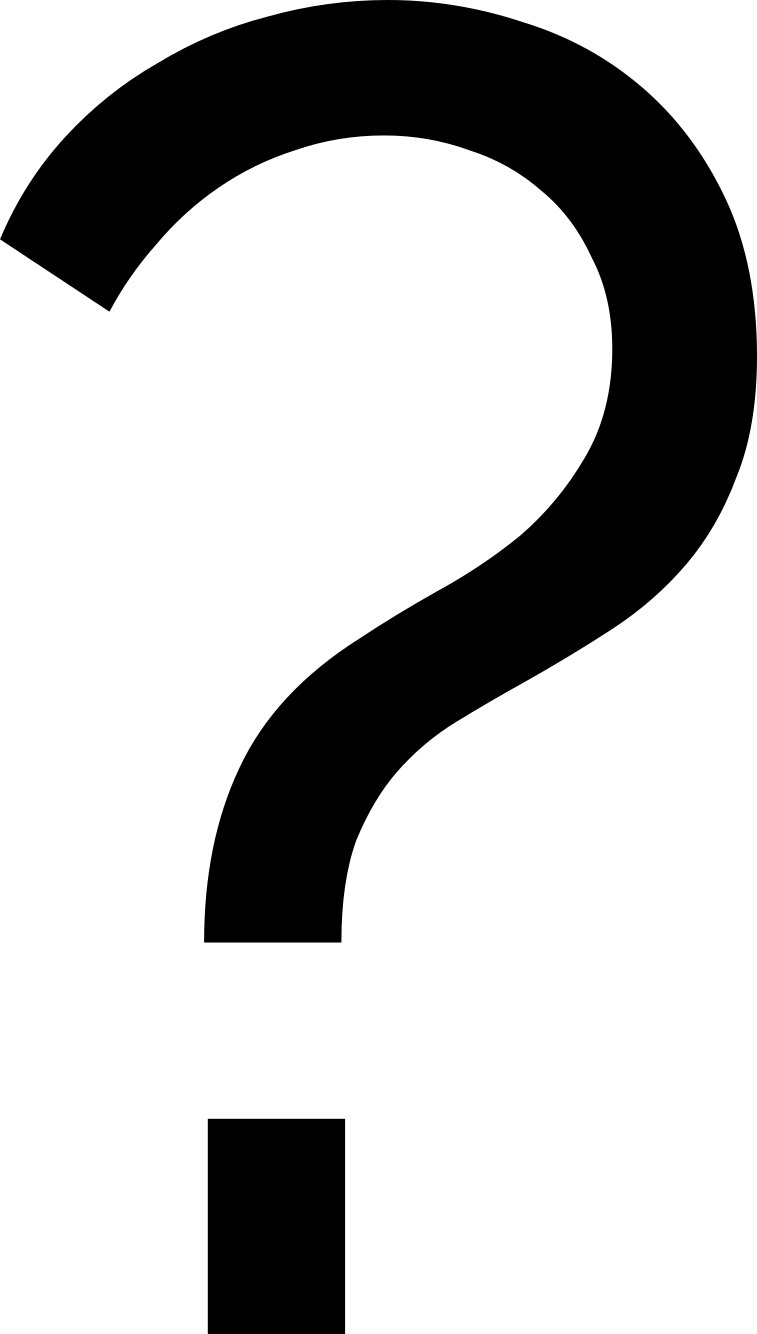
\includegraphics[width = 0.07\textwidth]{question.png}};
      \node[align=left, xshift=3cm] at (image3.east) {\bf Why do we need uncertainty \\ \bf quantification and what is it};
    \end{tikzpicture}

  \pause

  \begin{tikzpicture}[remember picture, overlay, font=\sffamily]
  \node [align=left, xshift=-0.25\textwidth,yshift=-0.05\textheight] (image1) at (current page.center)
      {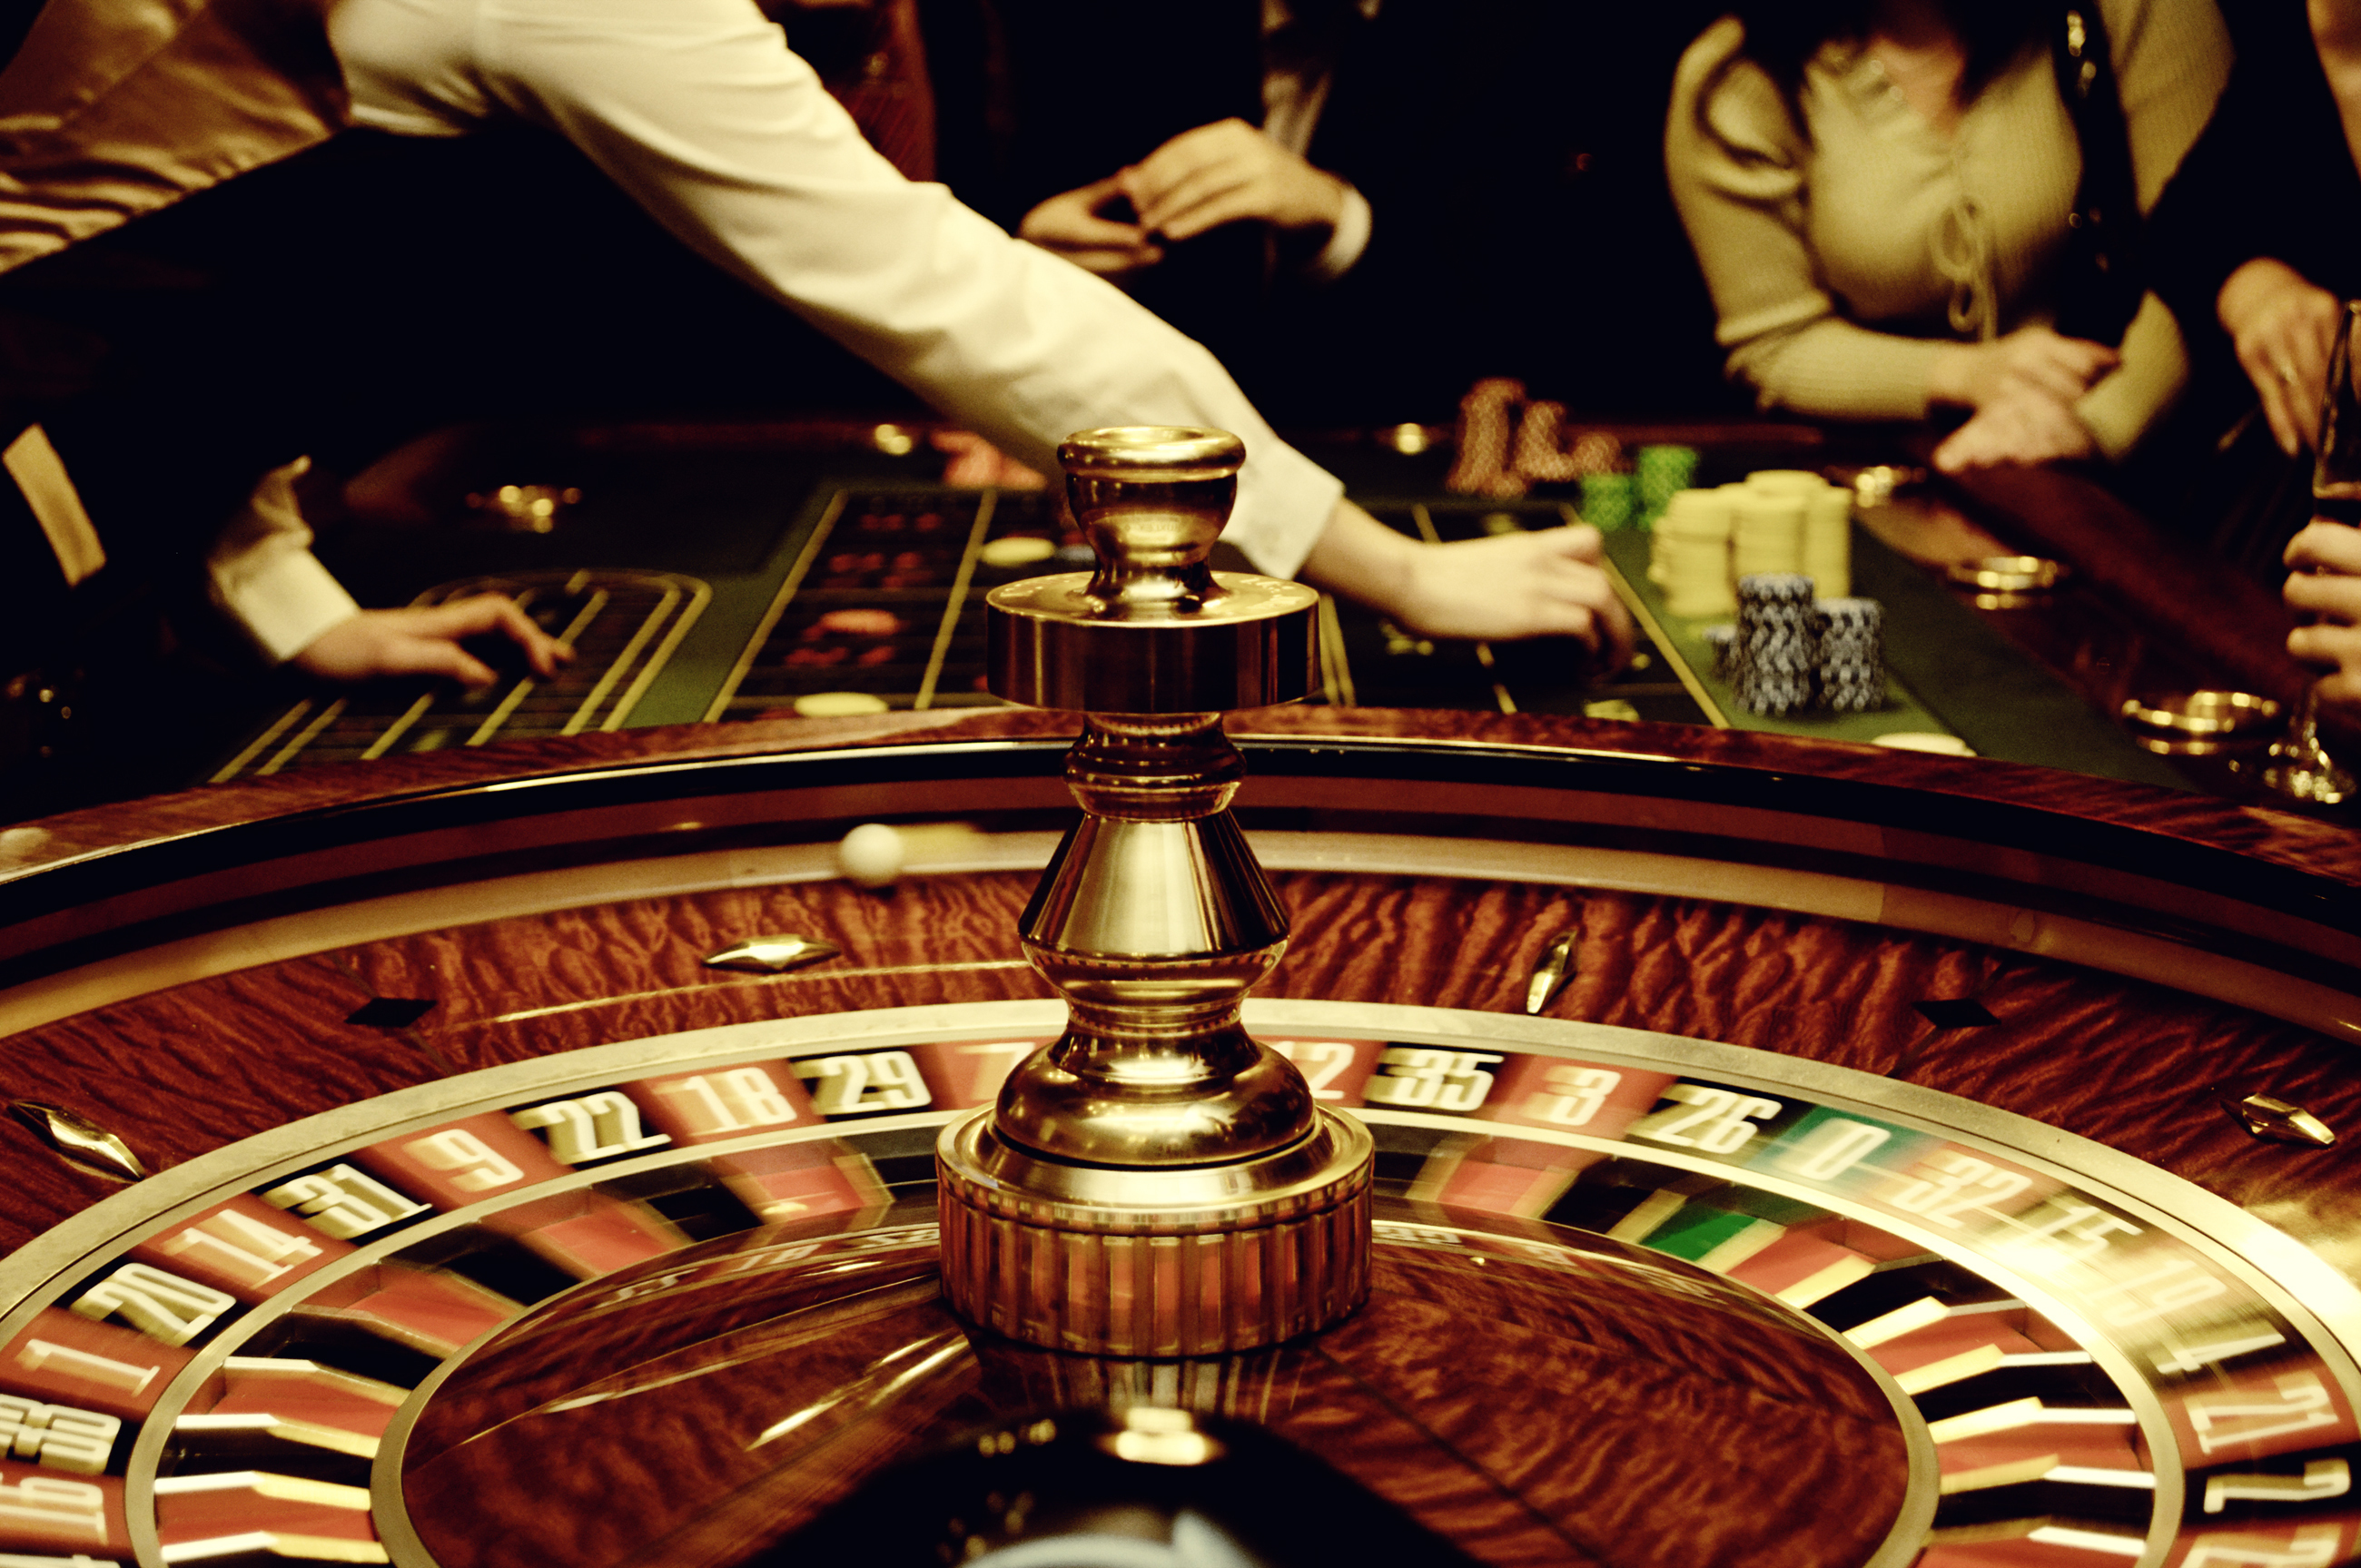
\includegraphics[width = 0.3\textwidth]{casino.jpg}};
  \node[align=left, xshift=2.5cm] at (image1.east) {\bf How to perform an \\ \bf uncertainty quantification};
  \end{tikzpicture}

\pause


    \begin{tikzpicture}[remember picture, overlay, font=\sffamily]
      \node [align=left, xshift=0\textwidth,yshift=-0.3\textheight] (image2) at (current page.center)
            {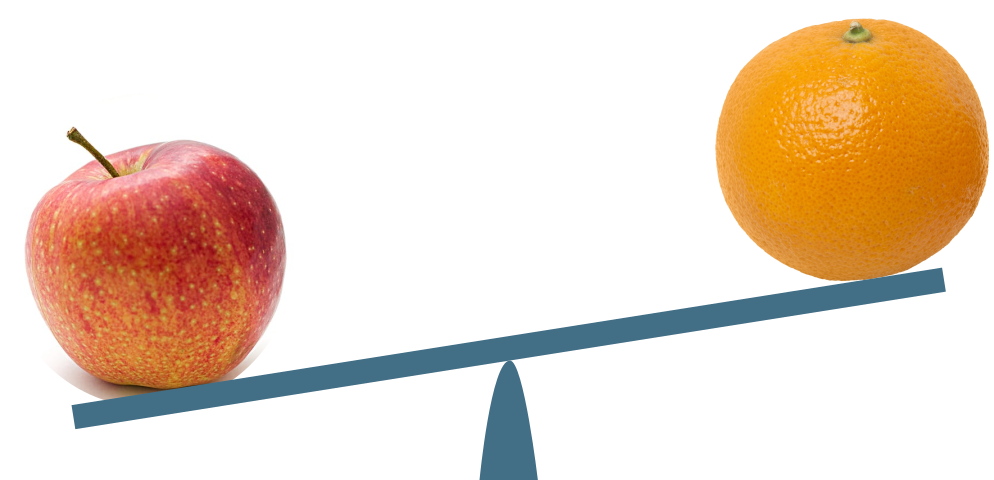
\includegraphics[width = 0.3\textwidth]{compare.png}};
      \node[align=left, xshift=2cm] at (image2.east) {\bf Comparison problems};
    \end{tikzpicture}

\end{frame}


%%%%%%%%%%%%%%%%%%%%%%%%%%%%%%%
%                             %
%   Define the problem        %
%                             %
%%%%%%%%%%%%%%%%%%%%%%%%%%%%%%%

%%%%%%%%%%%%%
%   Frame   %
%%%%%%%%%%%%%

\begin{frame}
  \only<1>{\fullimage{question.png}{.7}}
\end{frame}



%%%%%%%%%%%%%
%   Frame   %
%%%%%%%%%%%%%

\begin{frame}{Computational models contain parameters}
  % \[I = C_m\frac{{\mathrm d} V_m}{{\mathrm d} t}  + {\bf\color{logogrey}I_{K}} + {\bf\color{logoyellow}I_{Na}} + {\bf\color{logored}I_{l}}\]

  % \vspace{-5mm}
  \begin{figure}
    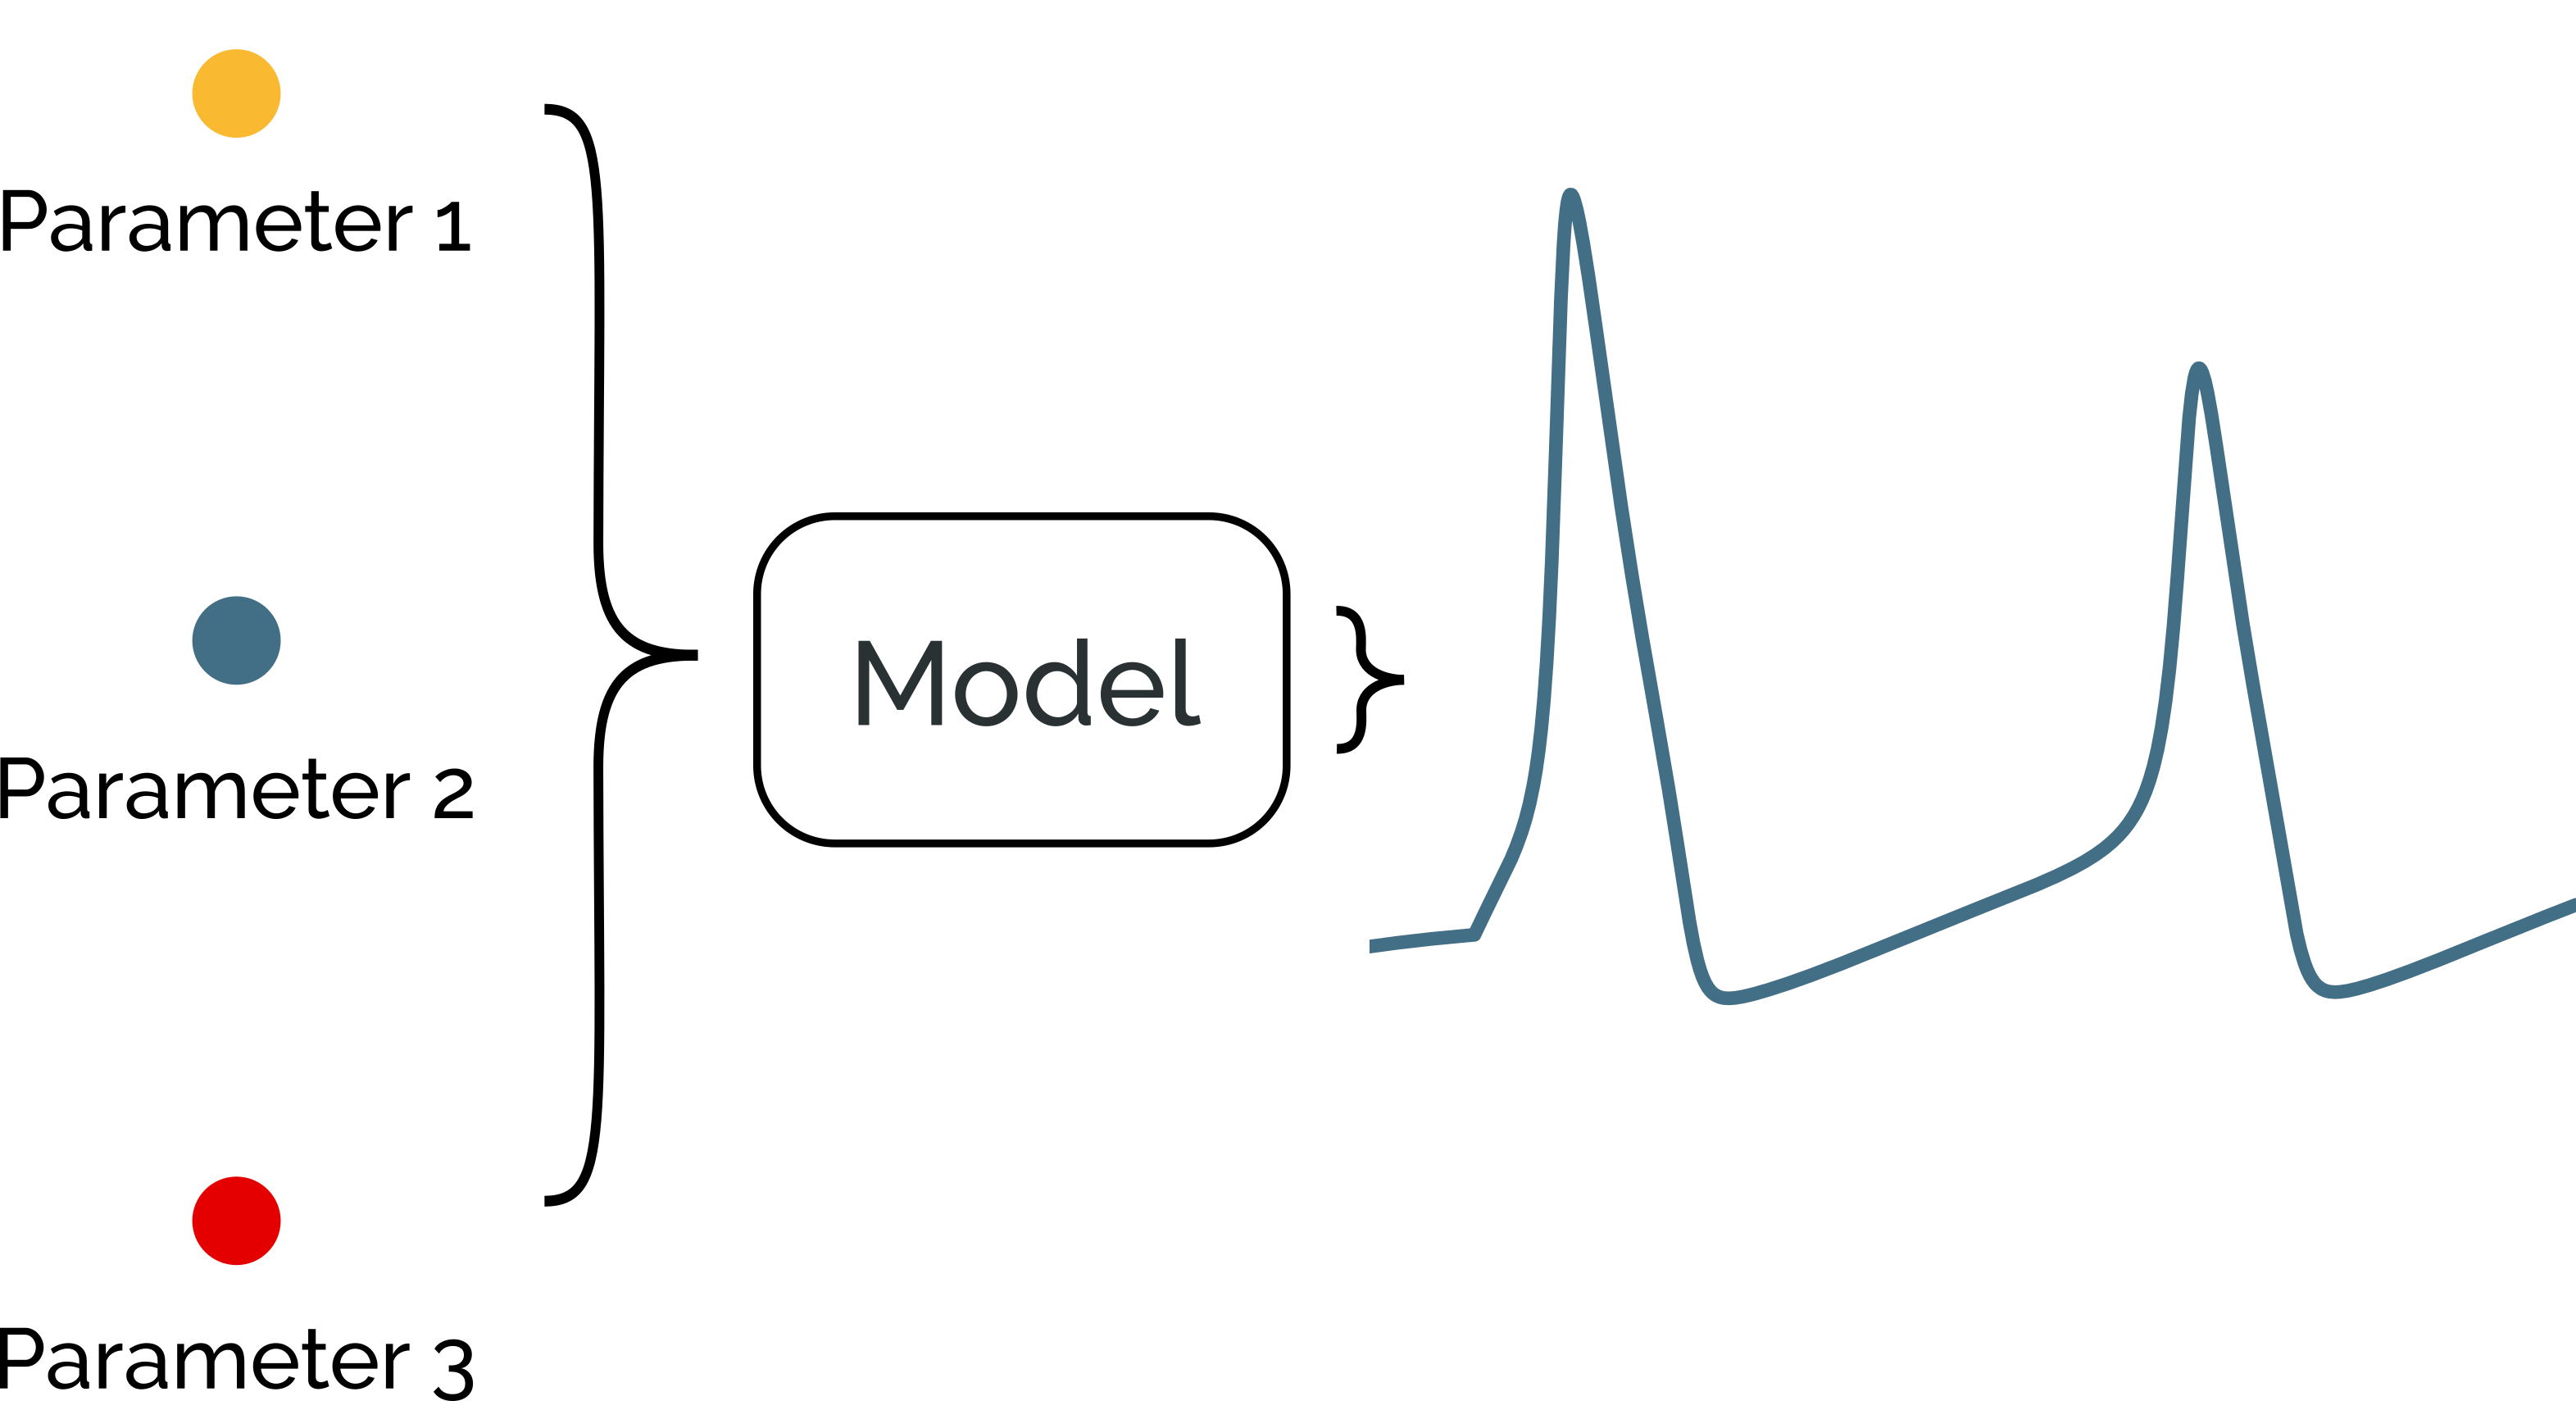
\includegraphics[width=\textwidth]{deterministic.png}
  \end{figure}

\end{frame}




\begin{frame}{The example we use is the Hodgkin-Huxley model}
  % \[I = C_m\frac{{\mathrm d} V_m}{{\mathrm d} t}  + I_{K} + I_{Na} +I_{l}\]
%  \only<1>{ \LARGE  \[I = C_m\frac{{\mathrm d} V_m}{{\mathrm d} t}  + {\bf\color{logogrey}I_{K}} + {\bf\color{logoyellow}I_{Na}} + {\bf\color{logored}I_{l}}\]}

\vspace{-7mm}

  \begin{figure}
    \onslide<2>{
\includegraphics[width=\textwidth]{hh_eq.png}}
  \end{figure}
\vspace{-19mm}

  \onslide<1->{ \LARGE  \[I = C_m\frac{{\mathrm d} V_m}{{\mathrm d} t}
               + {\bf\color{logogrey}\overline{g}_{K}}(\ldots)
               + {\bf\color{logoyellow}\overline{g}_{Na}}(\ldots)
               + {\bf\color{logored}\overline{g}_{l}}(\ldots) \]}

\end{frame}


%%%%%%%%%%%%%
%   Frame   %
%%%%%%%%%%%%%

\begin{frame}{The Hodgkin-Huxley model has three types of \\ion channels}

  \begin{figure}
    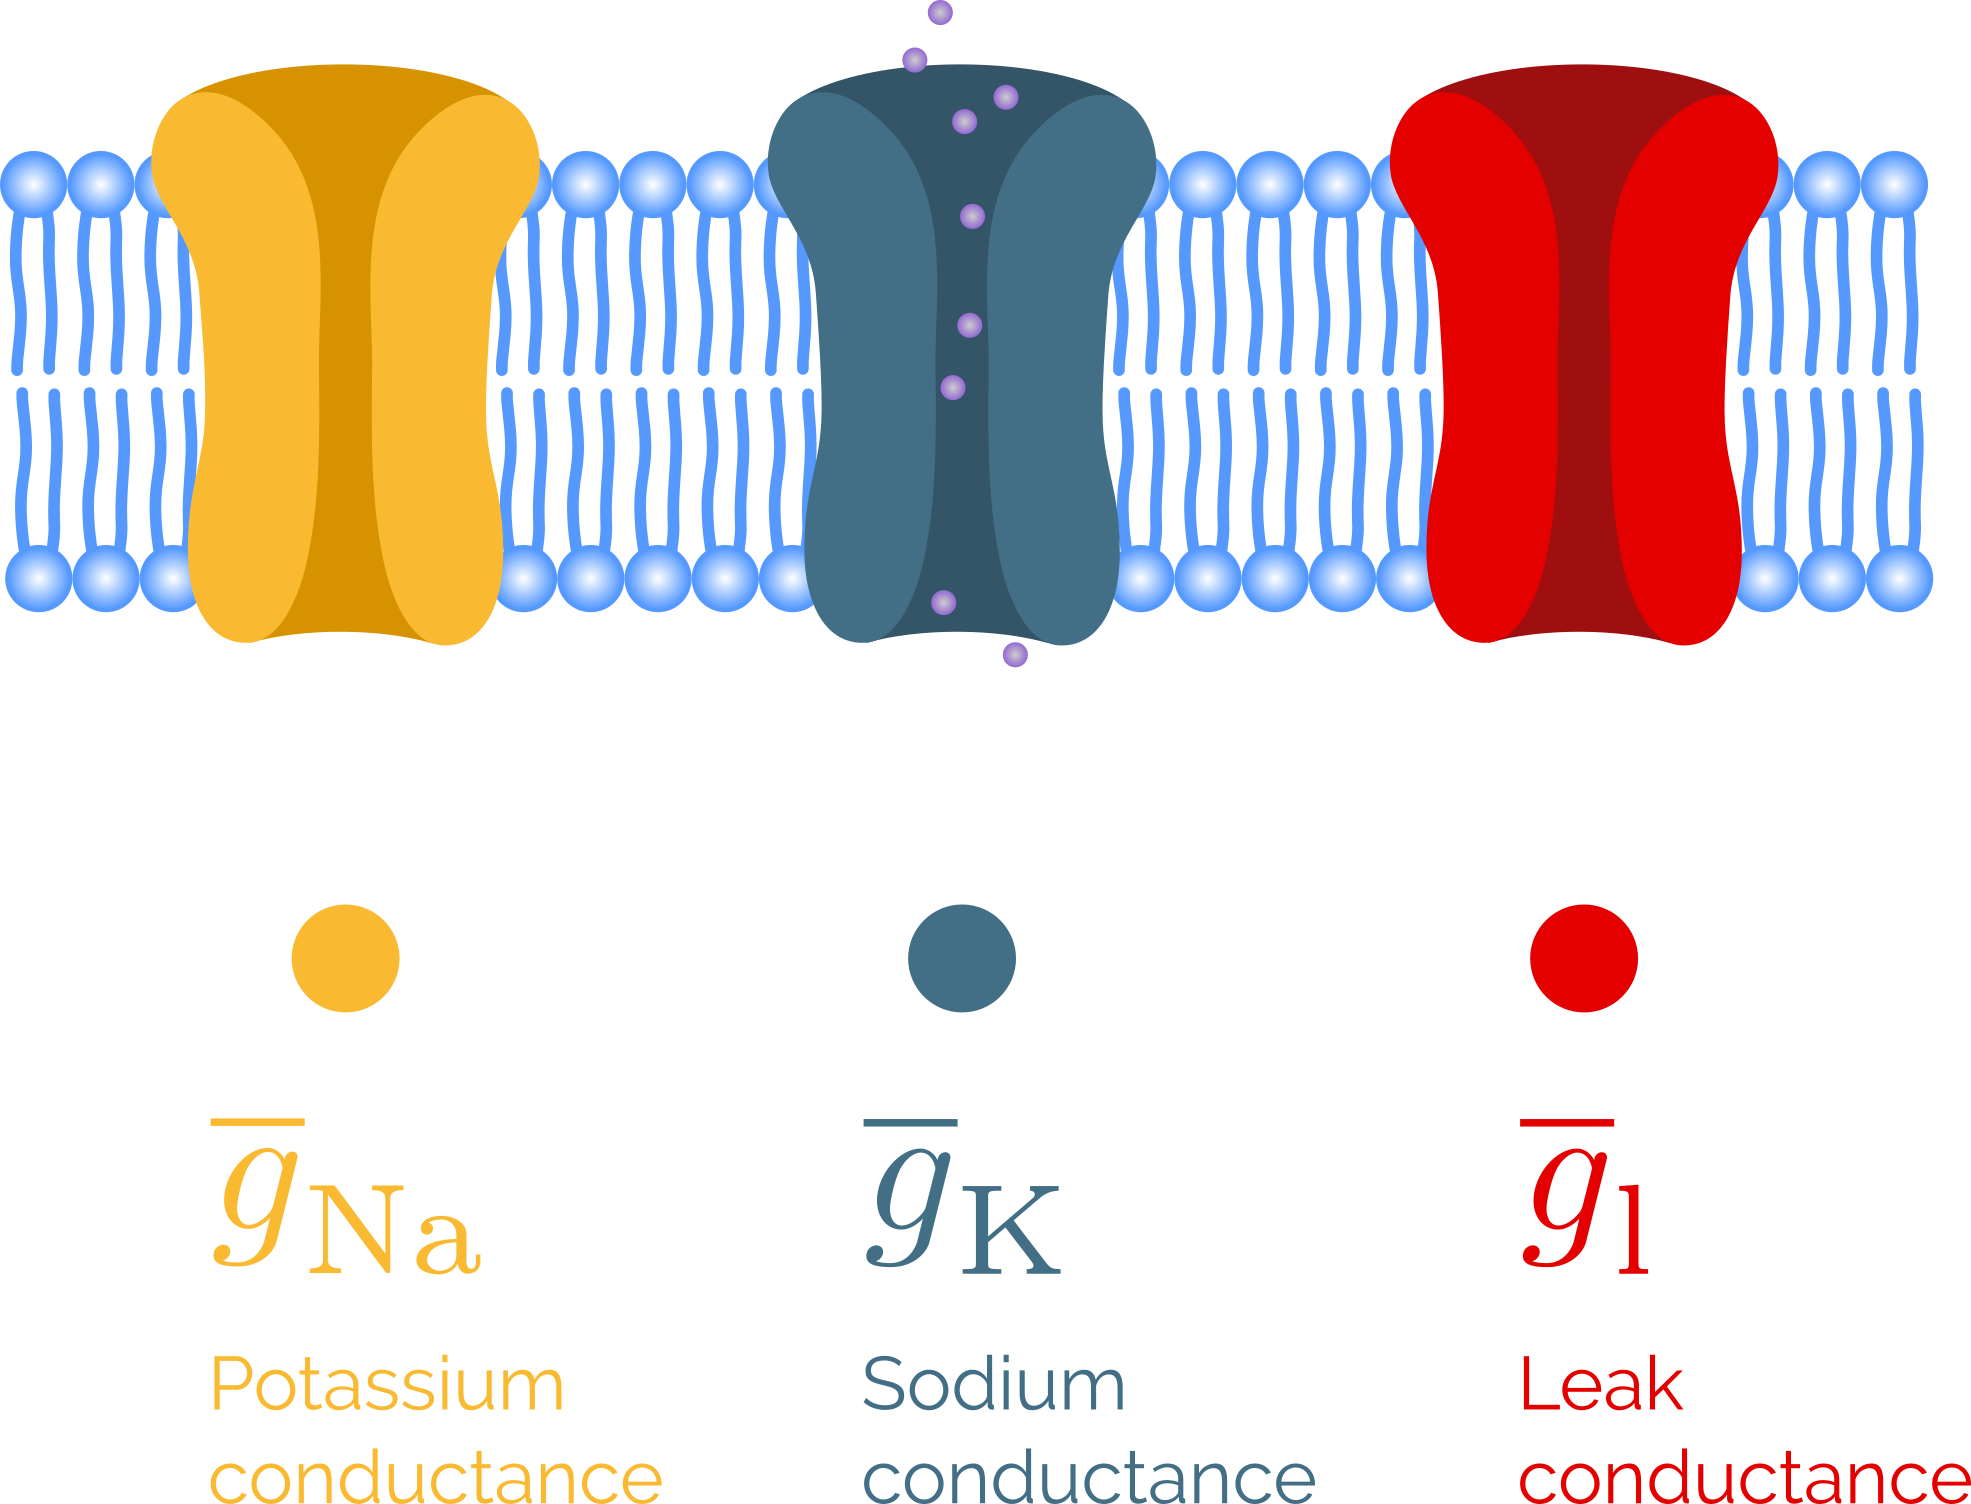
\includegraphics[width=\textwidth]{deterministic_channels.png}
  \end{figure}
\end{frame}


%%%%%%%%%%%%%
%   Frame   %
%%%%%%%%%%%%%

\begin{frame}{Membrane potential of the Hodgkin-Huxley model}
  \vspace{-5mm}
  \begin{figure}
    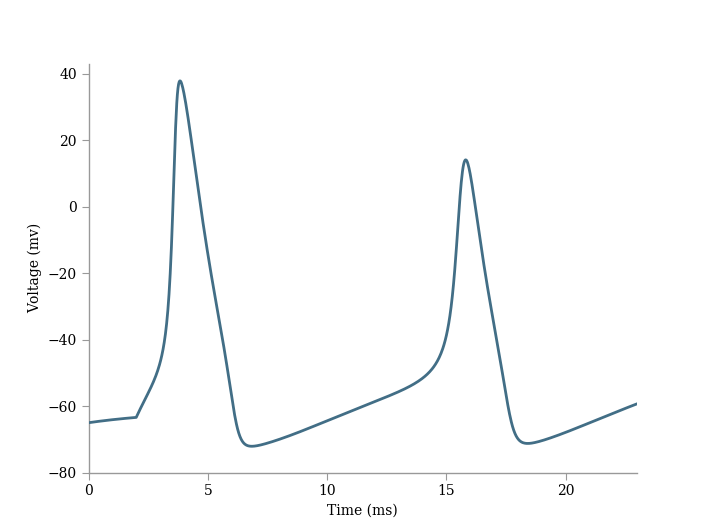
\includegraphics[width=\textwidth]{hh_single.png}
  \end{figure}

\end{frame}




%%%%%%%%%%%%%
%   Frame   %
%%%%%%%%%%%%%

\begin{frame}{Changing the parameters give different results}
% \[I = C_m\frac{{\mathrm d} V_m}{{\mathrm d} t}  + {\bf\color{logogrey}I_{K}} + {\bf\color{logoyellow}I_{Na}} + {\bf\color{logored}I_{l}}\]
\[I = C_m\frac{{\mathrm d} V_m}{{\mathrm d} t}
               + {\bf\color{logogrey}\overline{g}_{K}}(\ldots)
               + {\bf\color{logoyellow}\overline{g}_{Na}}(\ldots)
               + {\bf\color{logored}\overline{g}_{l}}(\ldots) \]

  \vspace{-5mm}
  \begin{figure}
    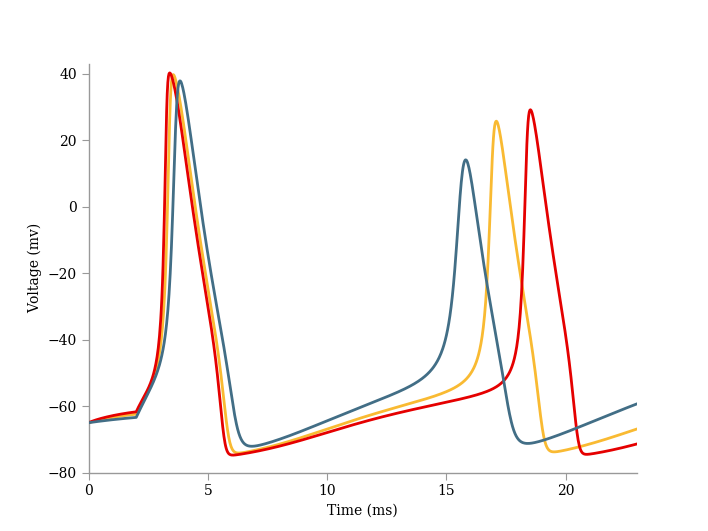
\includegraphics[height=0.7\textheight]{hh.png}
  \end{figure}

\end{frame}

% %%%%%%%%%%%%%
% %   Frame   %
% %%%%%%%%%%%%%

% \begin{frame}{Problem: The parameters are uncertain}
%   \begin{figure}
%     \only<1>{\includegraphics[width=1\textwidth]{not_deterministic.png}}
%     \only<2>{\includegraphics[width=1\textwidth]{not_deterministic_distributions.png}}
%   \end{figure}

% \end{frame}


%%%%%%%%%%%%%
%   Frame   %
%%%%%%%%%%%%%

\begin{frame}{The parameters do not have exact fixed values}
  \begin{figure}
    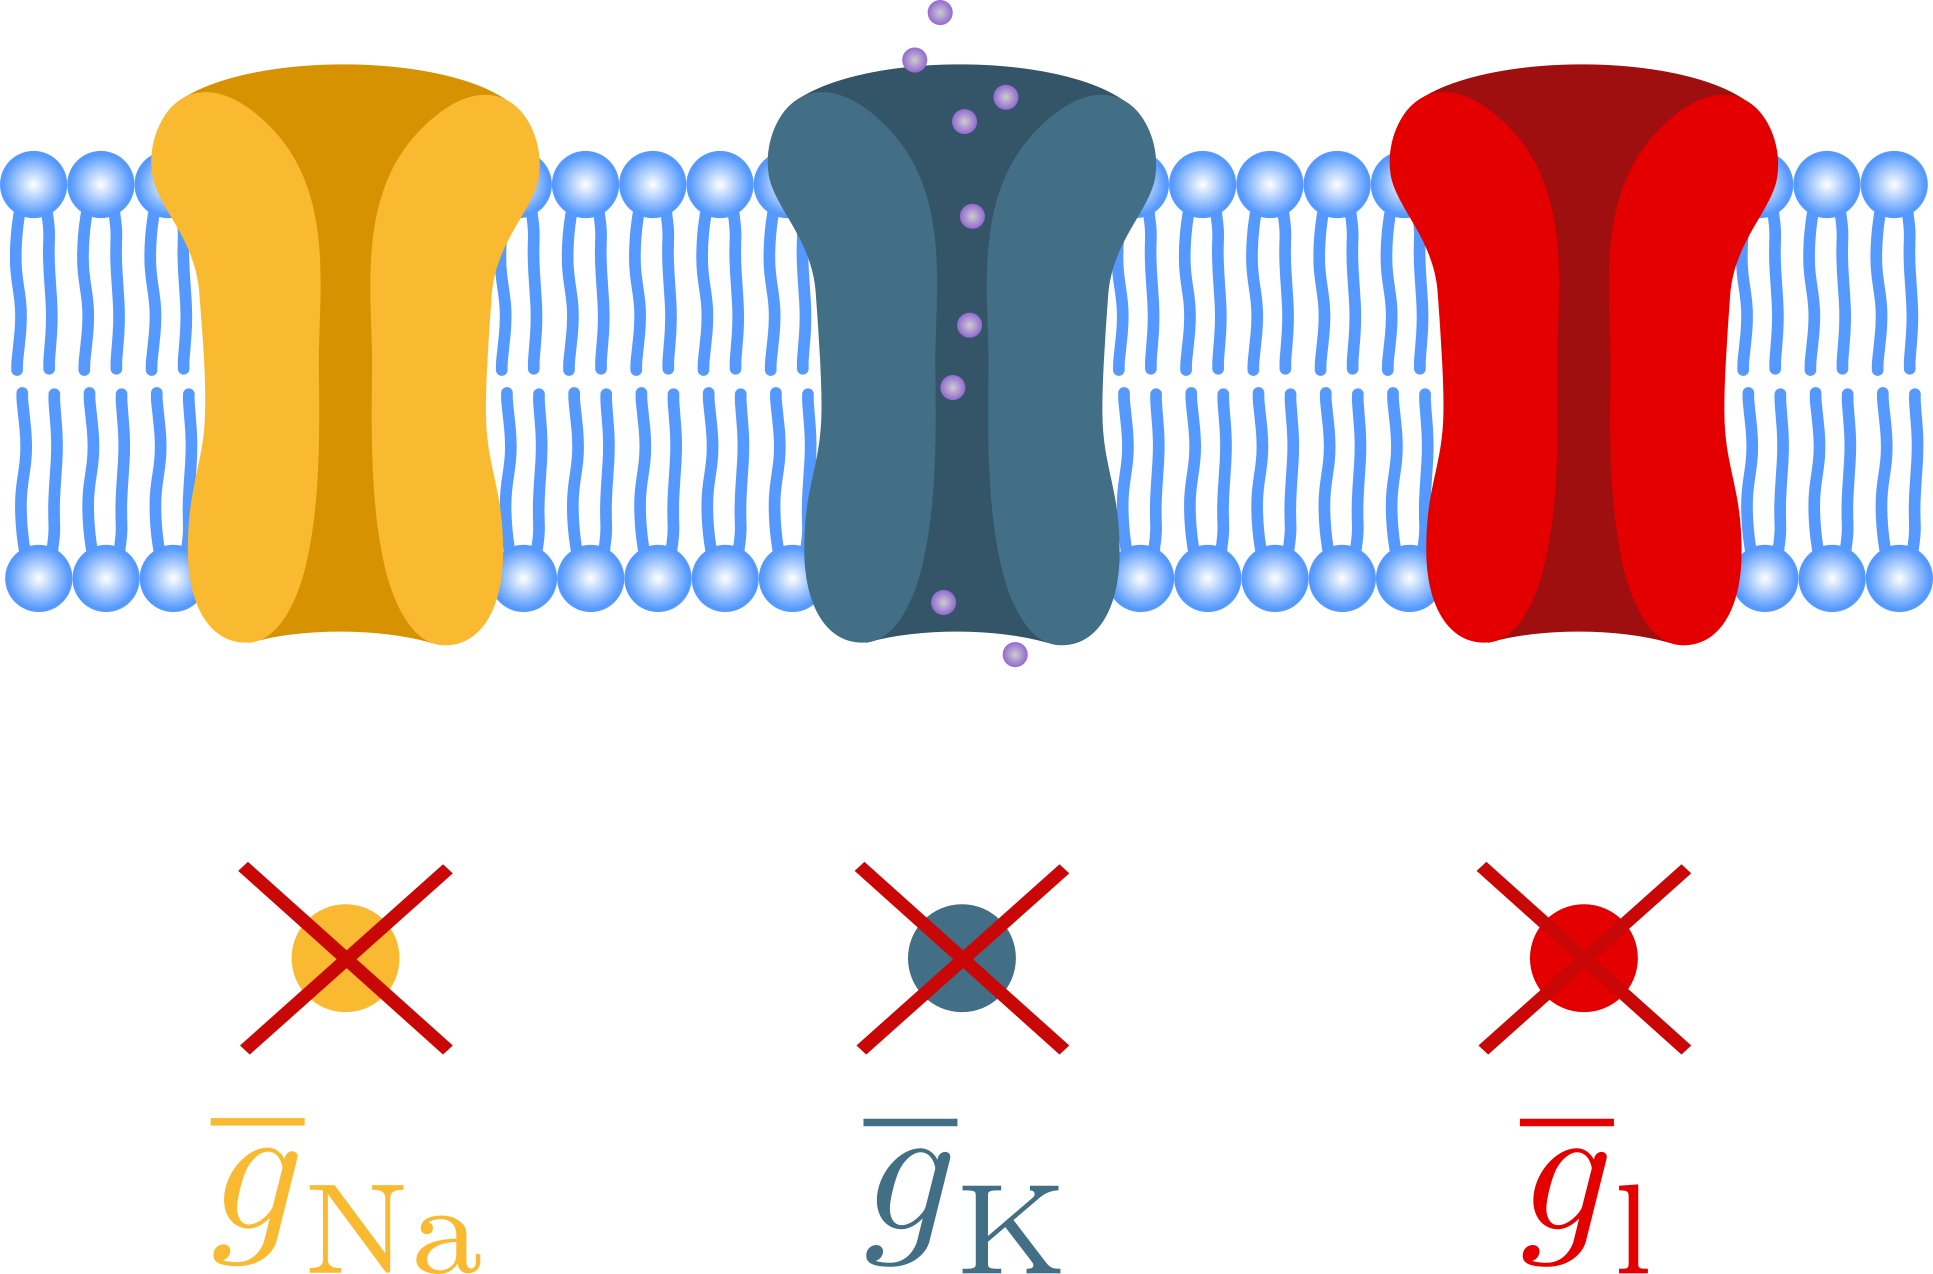
\includegraphics[width=1\textwidth]{not_deterministic_channels.png}
  \end{figure}

\end{frame}



%%%%%%%%%%%%%
%   Frame   %
%%%%%%%%%%%%%

% \begin{frame}[plain]{\color{black}Measurement uncertainty}

% \begin{tikzpicture}[remember picture, overlay]
%   \node[anchor = center] (image) at (current page.center) {\includegraphics[scale=0.38]{eeg.jpg}};
%   \node[align = left, xshift=0.4cm, yshift=-0.4cm] at (current page.135) {\bf Measurement uncertainty};
% \end{tikzpicture}

% \end{frame}

\begin{frame}{Measurement uncertainty}

  \begin{figure}
    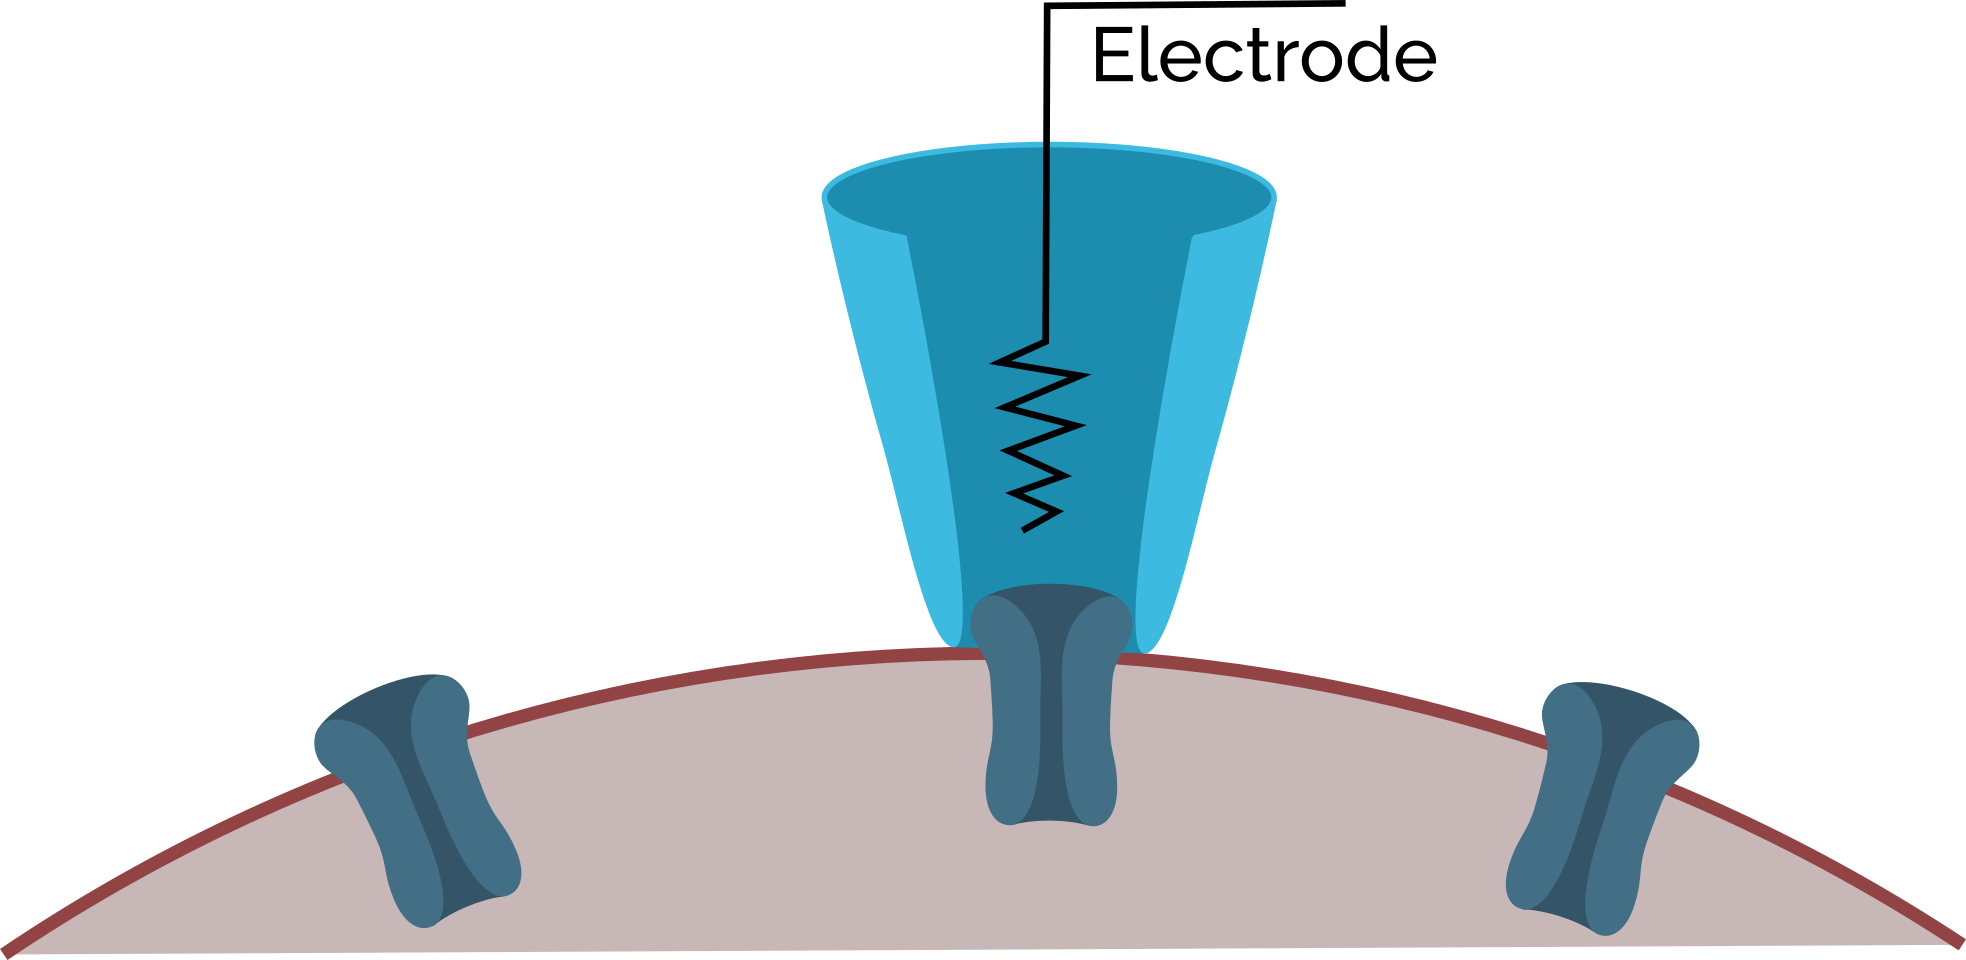
\includegraphics[width=1\textwidth]{patch_clamp.png}
  \end{figure}

\end{frame}


%%%%%%%%%%%%%
%   Frame   %
%%%%%%%%%%%%%

\begin{frame}{Biological variability: parameters change \\ over time }
  \begin{figure}
    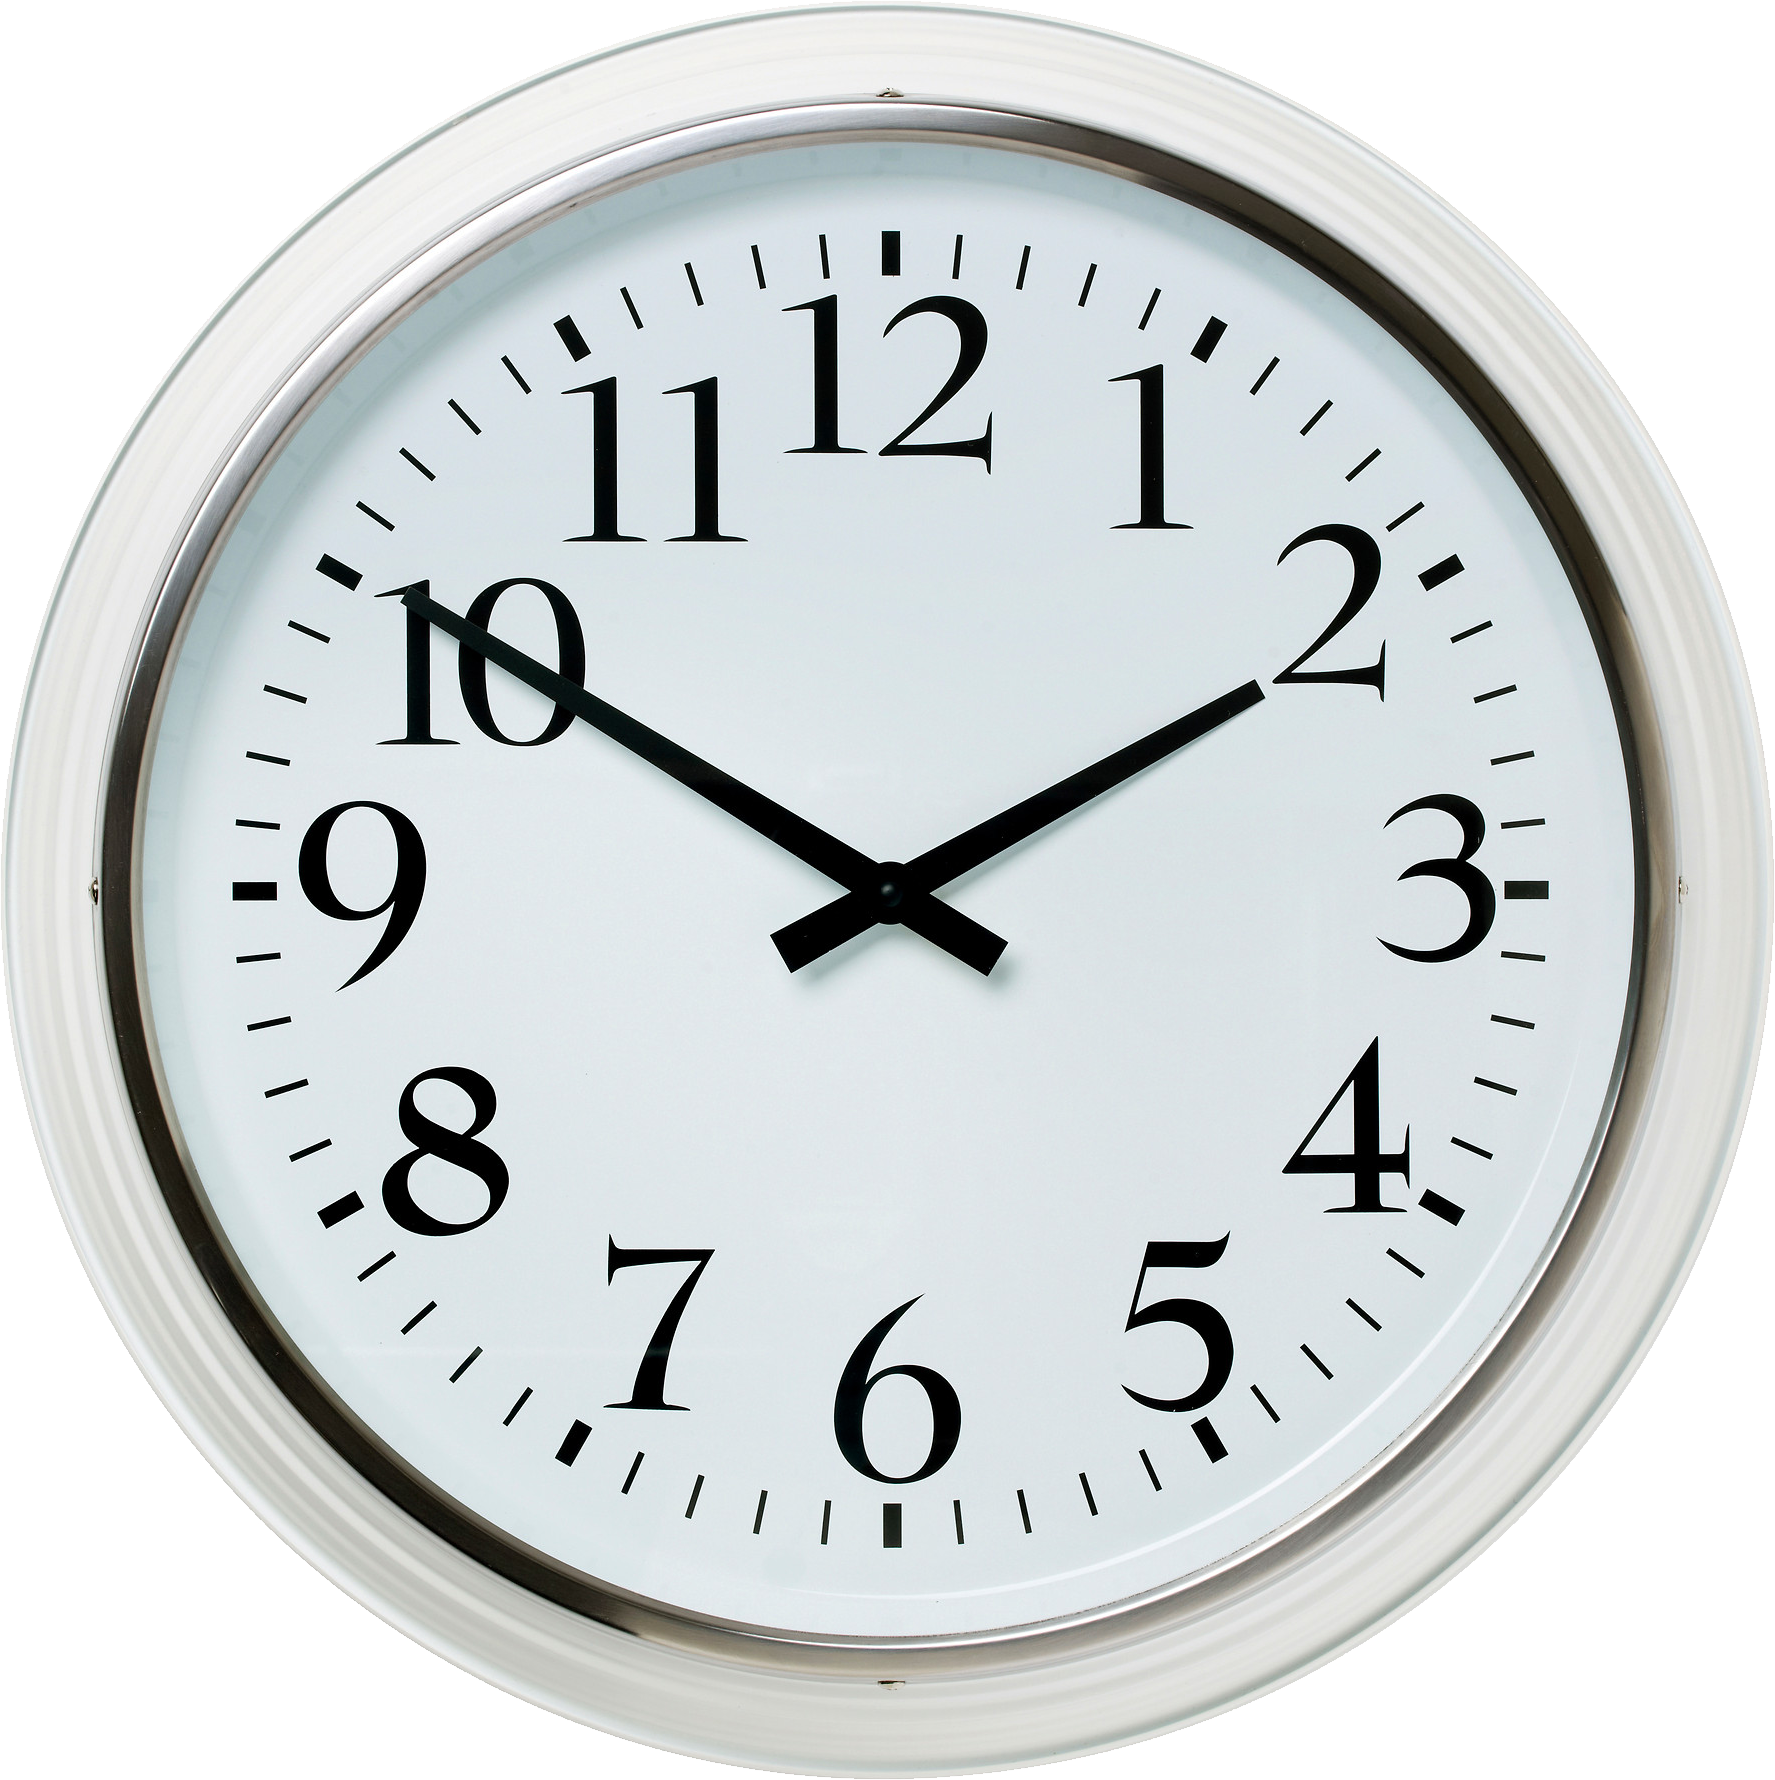
\includegraphics[height=0.7\textheight]{time.png}

  \end{figure}

\end{frame}


%%%%%%%%%%%%%
%   Frame   %
%%%%%%%%%%%%%

\begin{frame}{Biological variability: parameters vary within \\ a neuron}
  \begin{figure}
    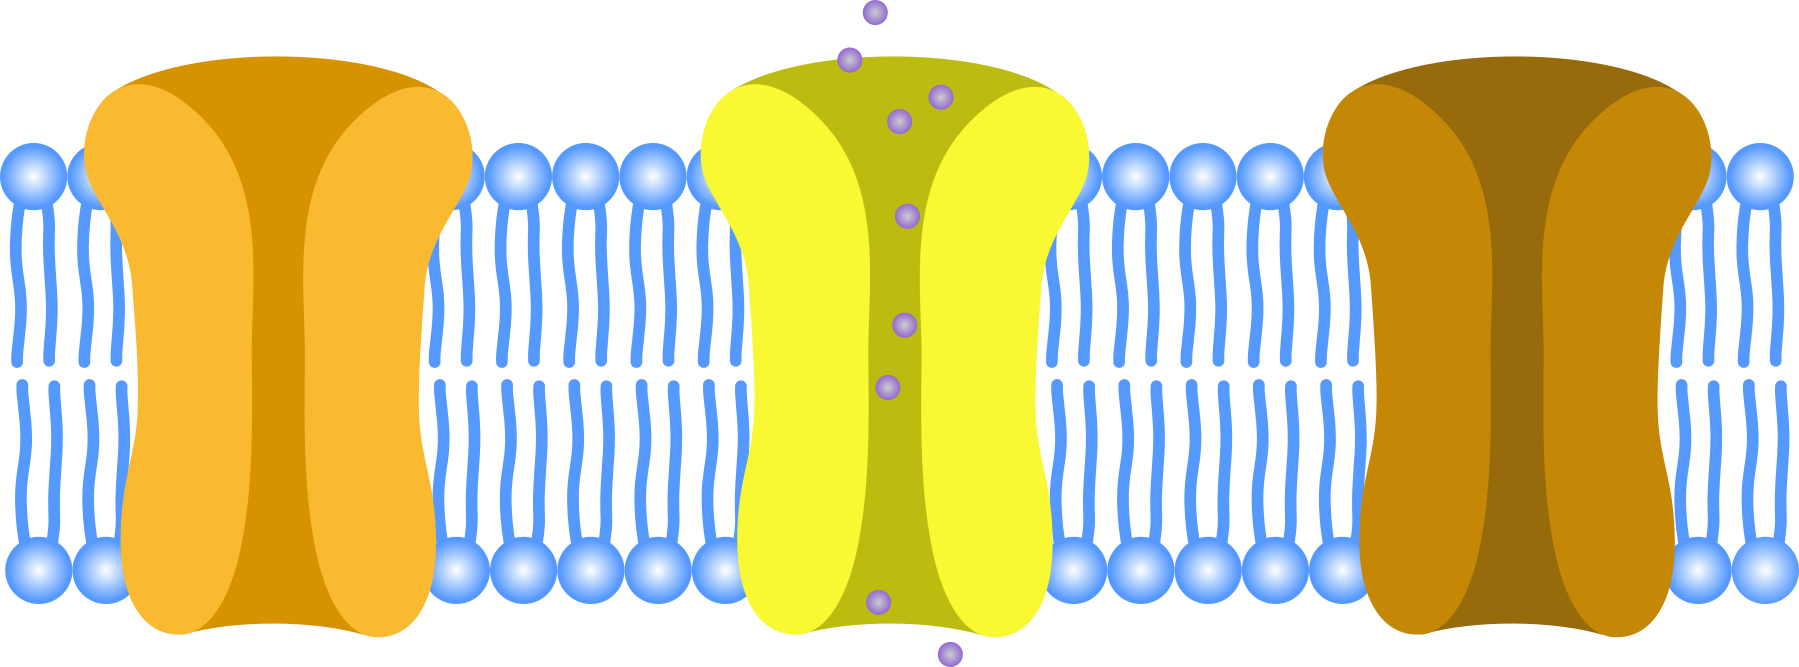
\includegraphics[width=1\textwidth]{channels_diverse.png}

  \end{figure}

\end{frame}

%%%%%%%%%%%%%
%   Frame   %
%%%%%%%%%%%%%

\begin{frame}{Biological variability: parameters vary between several neurons of the same type}
  \begin{figure}
    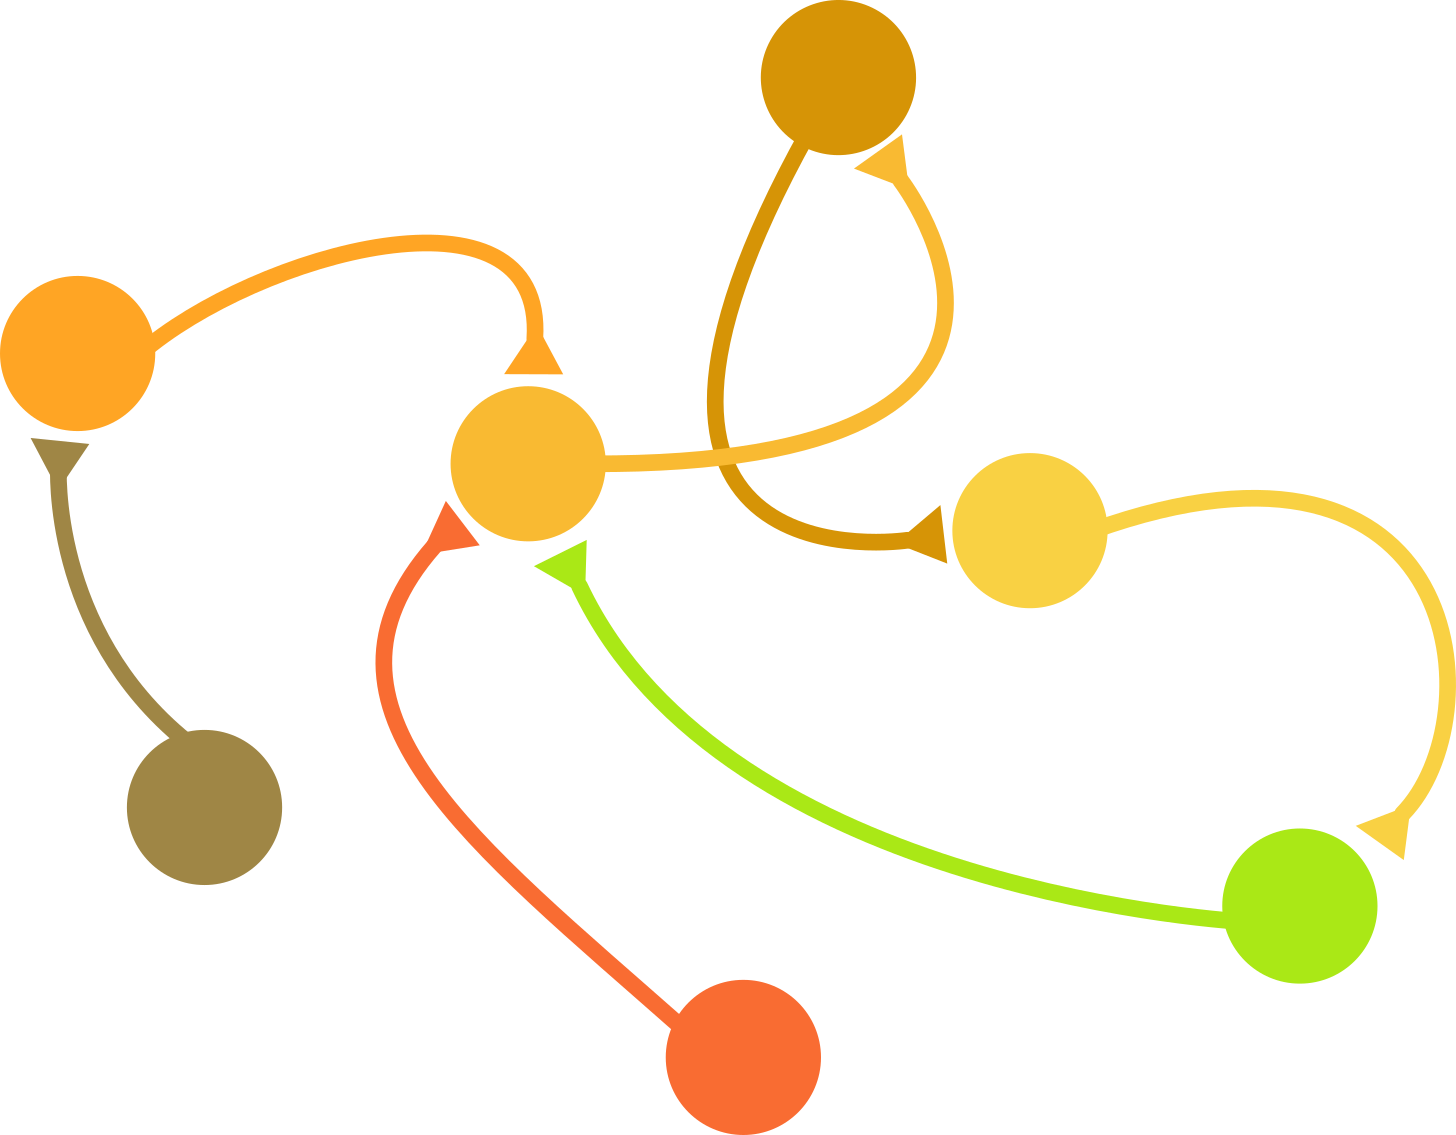
\includegraphics[height=0.7\textheight]{network.png}
  \end{figure}

\end{frame}


% %%%%%%%%%%%%%
% %   Frame   %
% %%%%%%%%%%%%%

% \begin{frame}{Biological variability}

% \begin{minipage}[t]{0.4\textwidth}
%   The parameters:
%   \begin{itemize}[<+->]
%     \item change over time
%     \item vary within a neuron
%     \item vary between several neurons of the same type
%   \end{itemize}
% \end{minipage}
% \hfill
% \begin{minipage}[t]{0.5\textwidth}
%   \begin{figure}
%     \only<1>{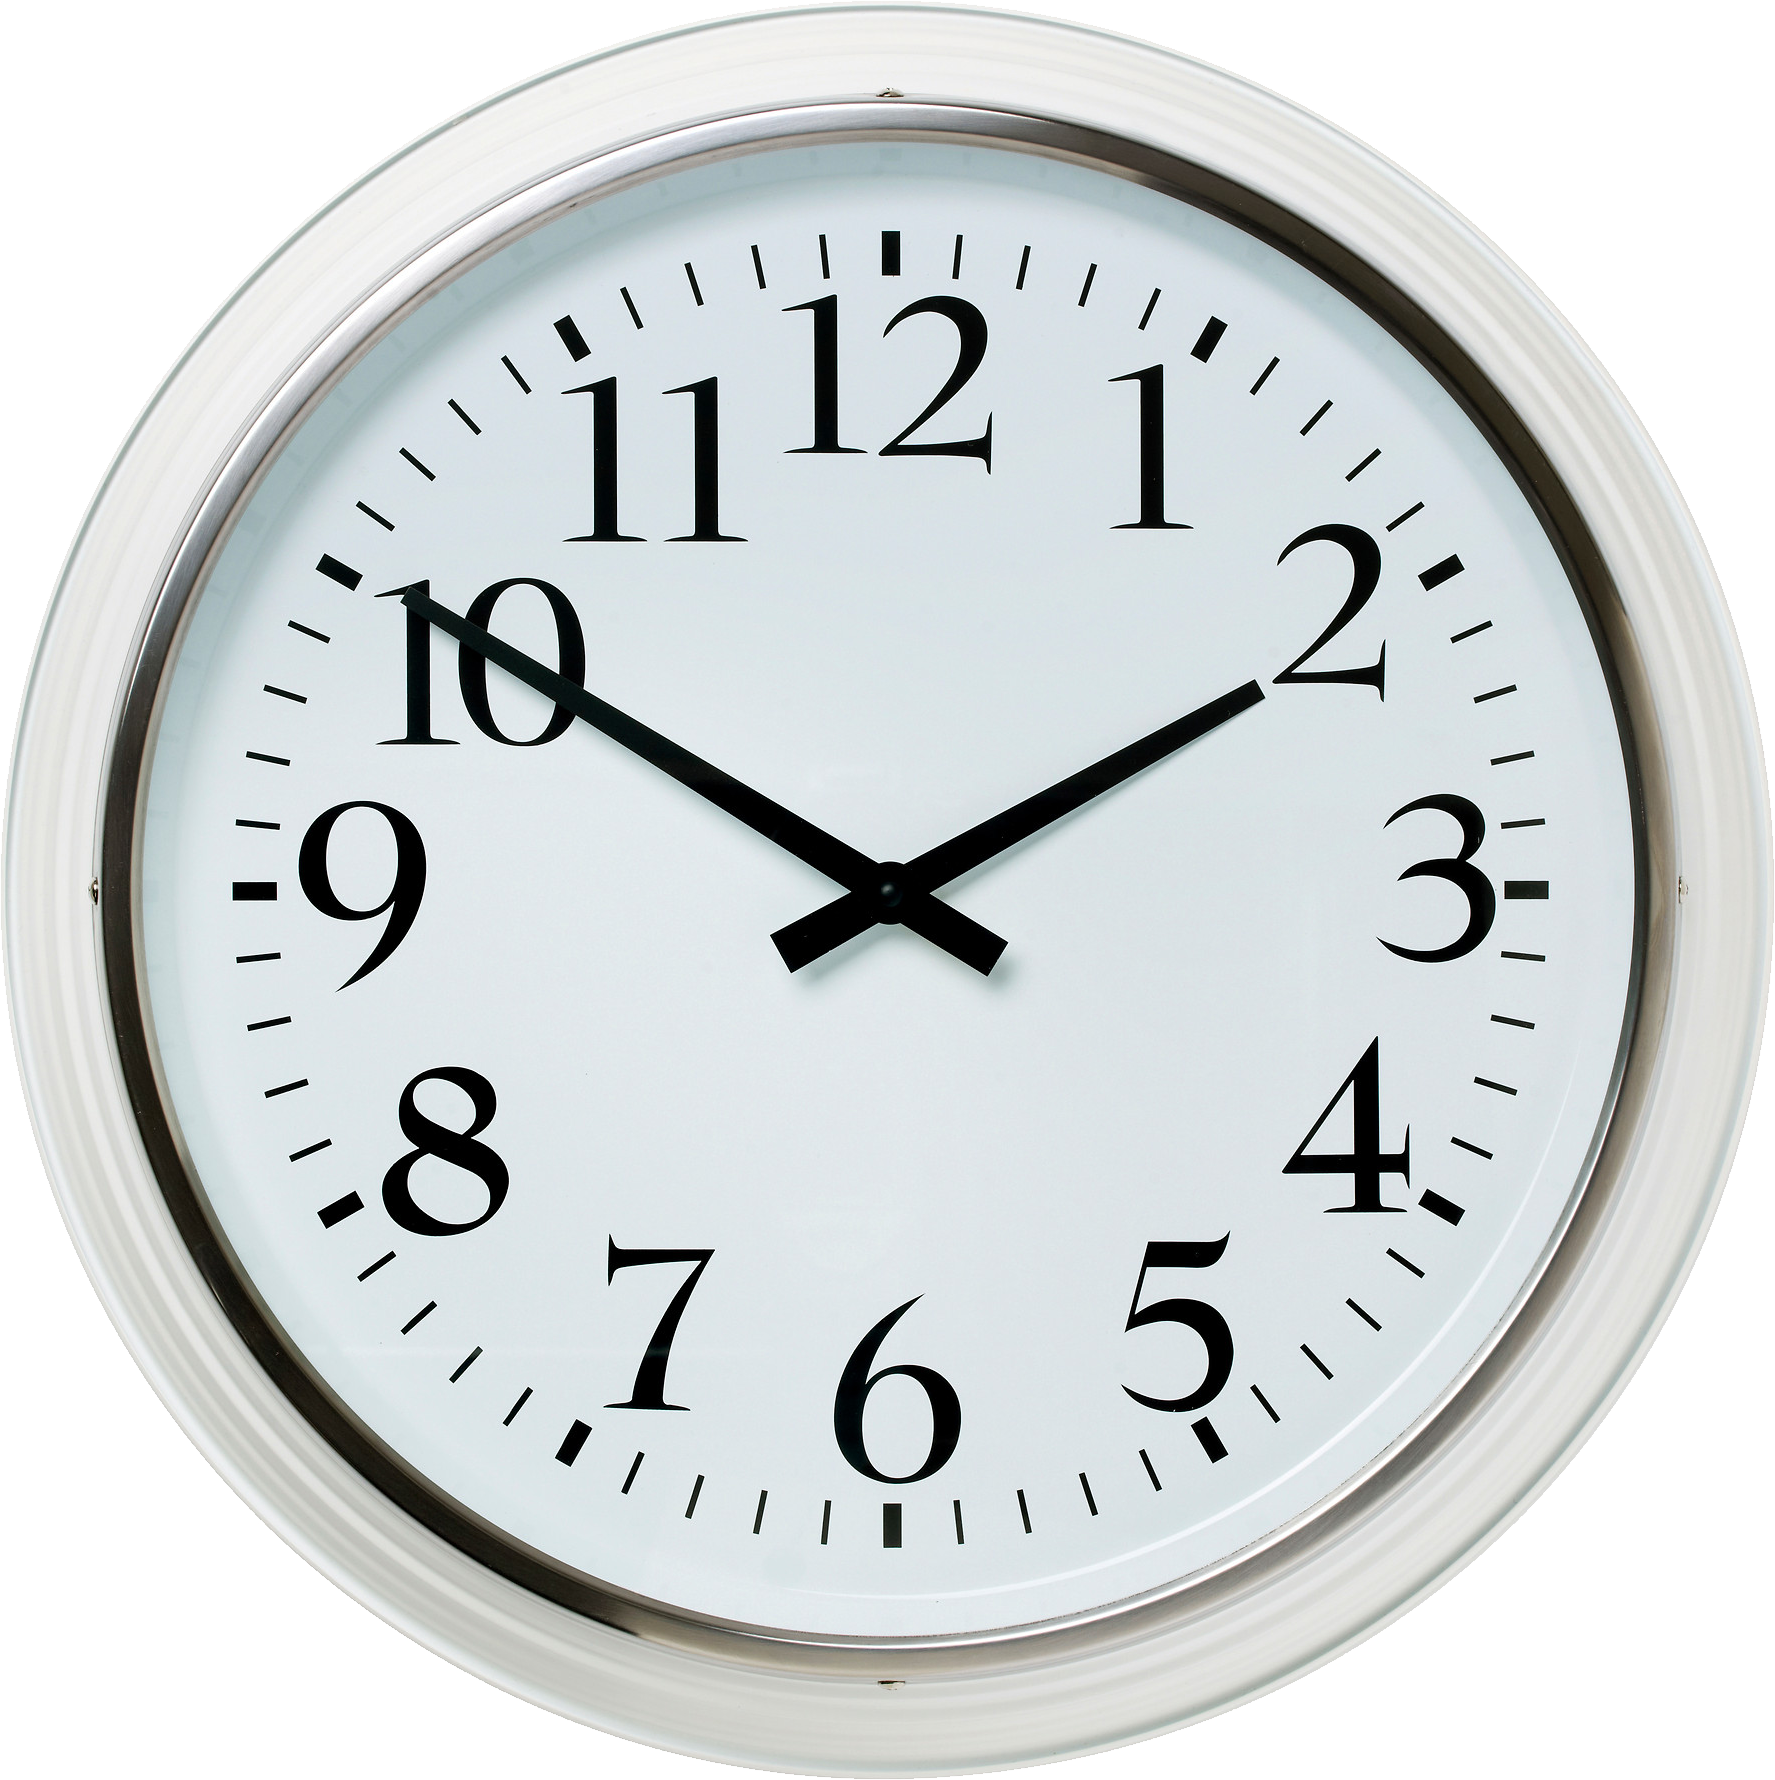
\includegraphics[width=1\textwidth]{time.png}}
%     \only<2>{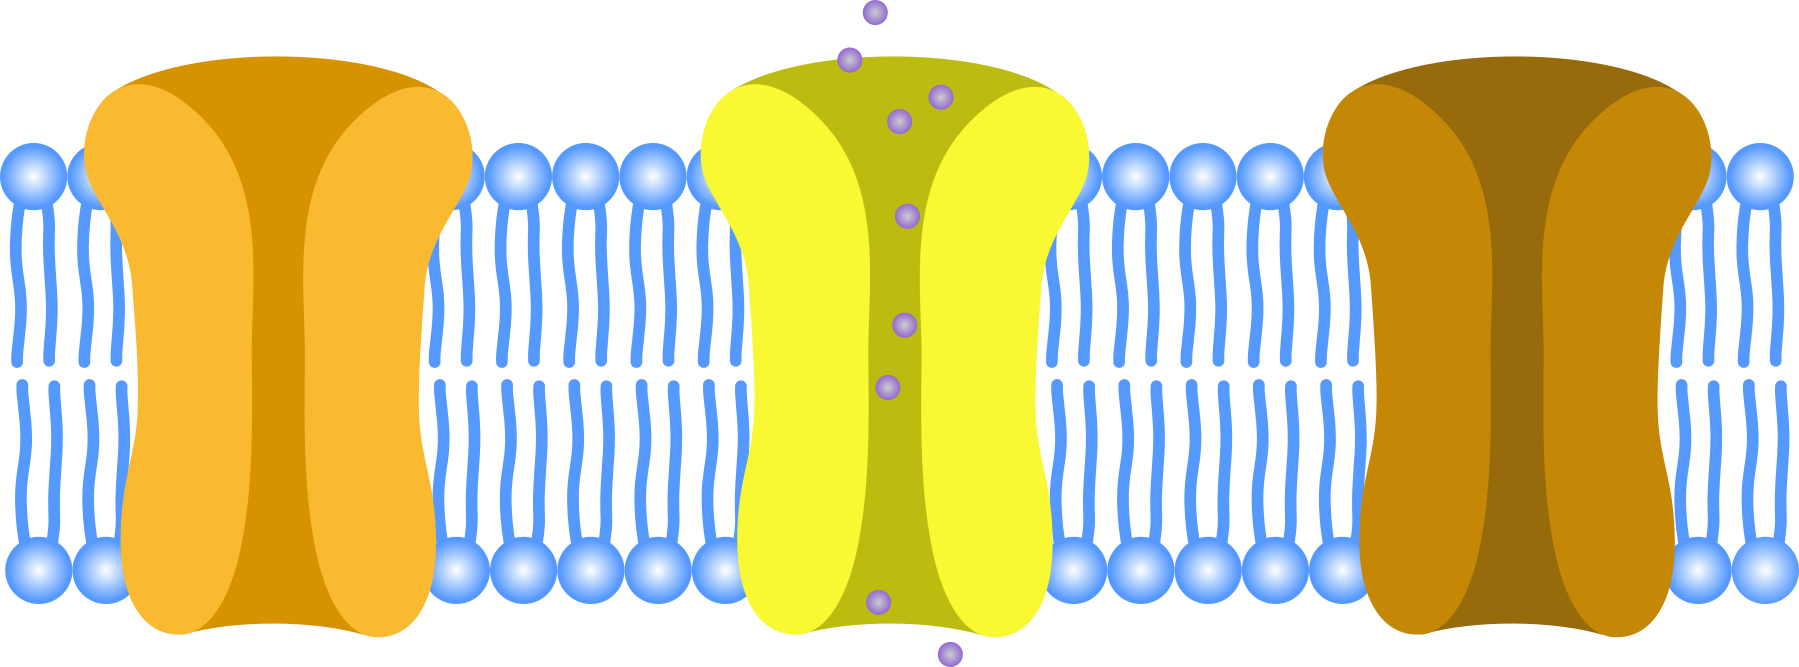
\includegraphics[width=1\textwidth]{channels_diverse.png}}
%     \only<3>{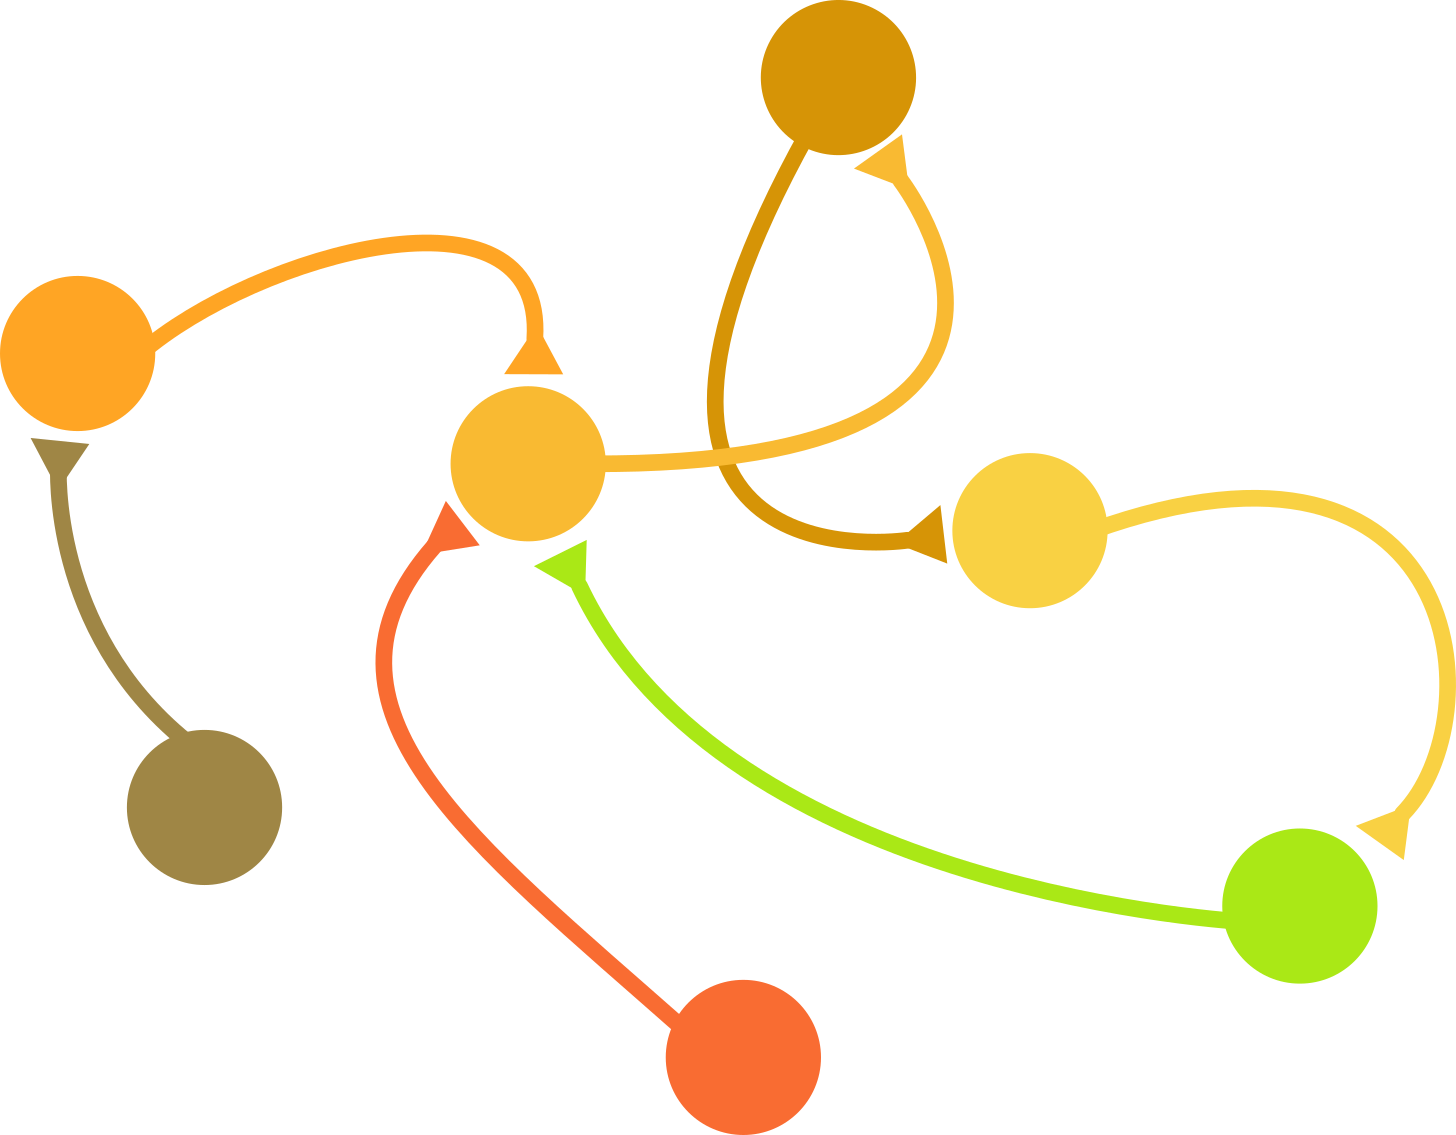
\includegraphics[width=1\textwidth]{network.png}}
%   \end{figure}
% \end{minipage}



% \end{frame}



%%%%%%%%%%%%%
%   Frame   %
%%%%%%%%%%%%%

\begin{frame}{Parameters are best described by distributions}
  \begin{figure}
    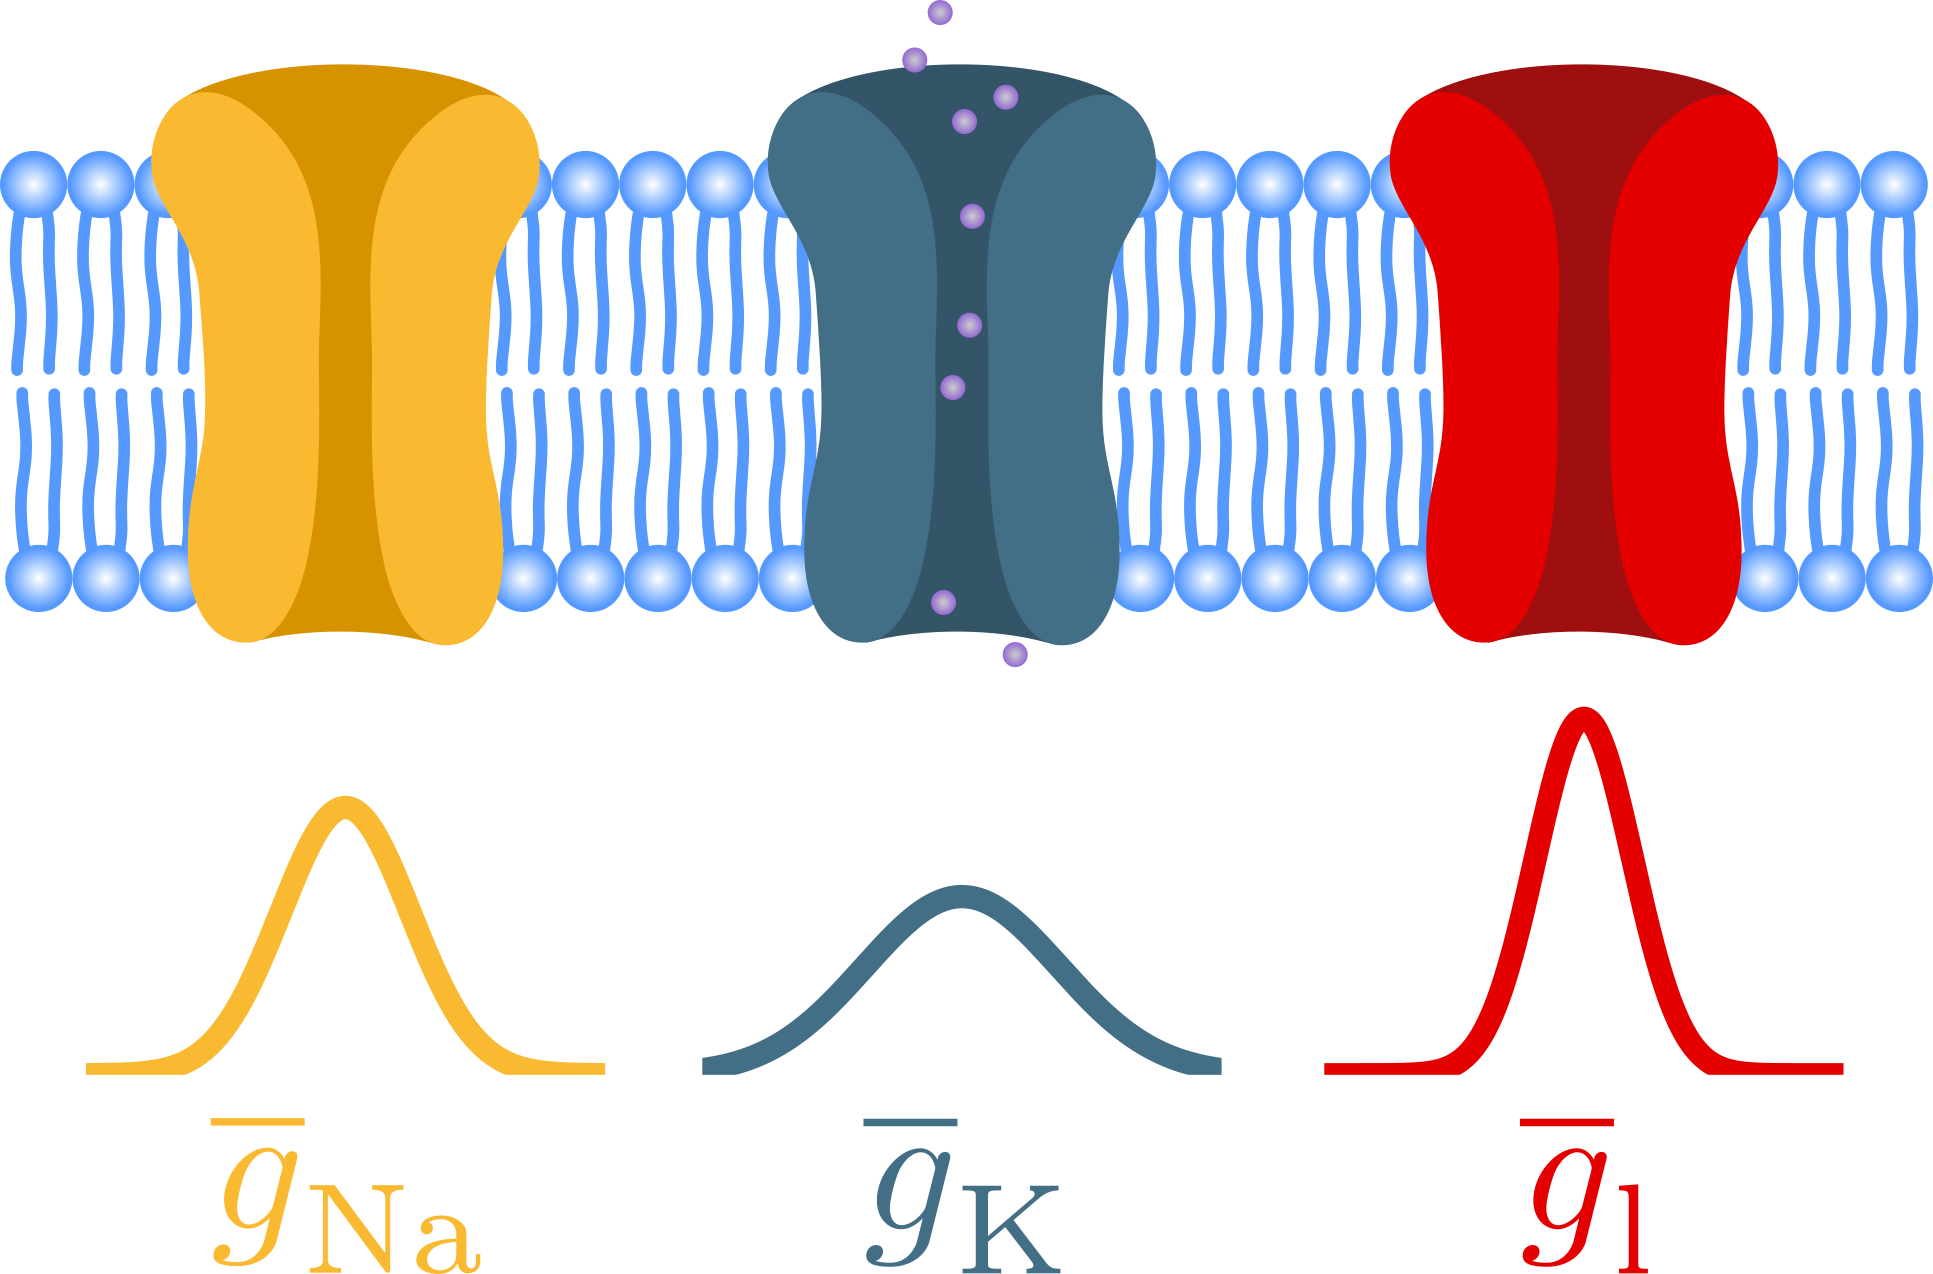
\includegraphics[width=1\textwidth]{distribution_channels.png}
  \end{figure}

\end{frame}


%%%%%%%%%%%%%
%   Frame   %
%%%%%%%%%%%%%

\begin{frame}
  \textbf{\Large{\color{myred}
  Uncertainty quantification} enables us to take the effects of
  uncertain parameters into account}

\end{frame}



%%%%%%%%%%%%%%%%%%%%%%%%%%%%%%%
%                             %
%   What is UQ                %
%                             %
%%%%%%%%%%%%%%%%%%%%%%%%%%%%%%%


%%%%%%%%%%%%%
%   Frame   %
%%%%%%%%%%%%%

\begin{frame}{Uncertainty quantification is the process of quantifying the effects of
              uncertain parameters}
  \begin{figure}
    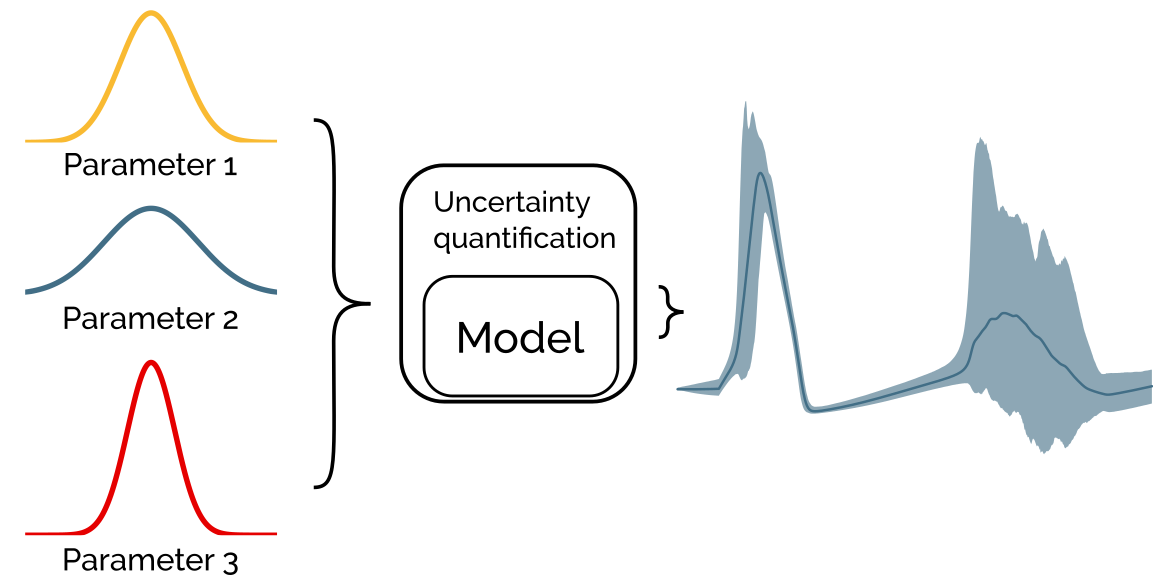
\includegraphics[width=1\textwidth]{probabalistic.png}
  \end{figure}

\end{frame}



%%%%%%%%%%%%%
%   Frame   %
%%%%%%%%%%%%%

\begin{frame}{90\% prediction interval of the \\ Hodgkin-Huxley model}
  \vspace{-5mm}
  \begin{figure}
    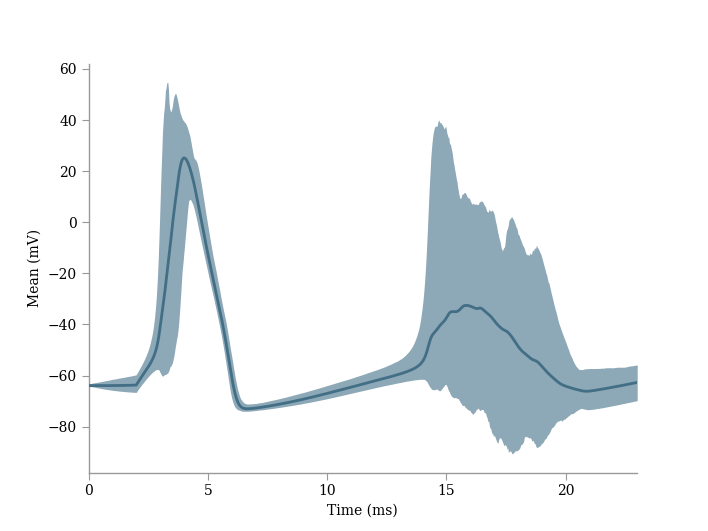
\includegraphics[width=1\textwidth]{hh_prediction.png}
  \end{figure}

\end{frame}



%%%%%%%%%%%%%
%   Frame   %
%%%%%%%%%%%%%

\begin{frame}{Mean and variance of the Hodgkin-Huxley model}
  \vspace{-5mm}
  \begin{figure}
    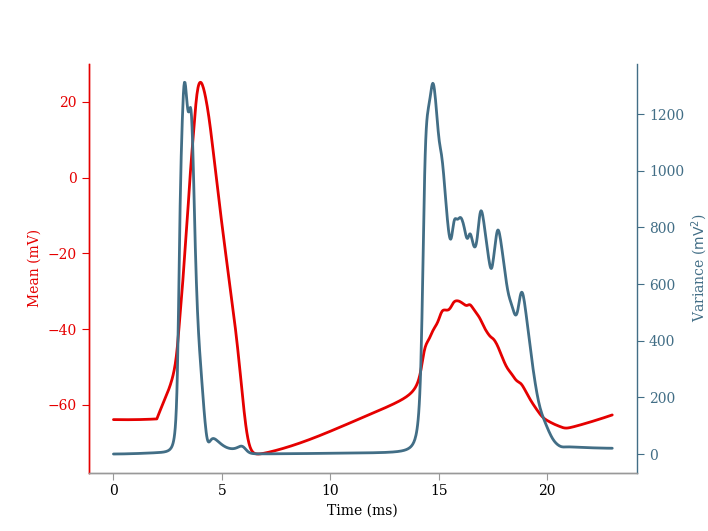
\includegraphics[width=1\textwidth]{hh_mean.png}
  \end{figure}

\end{frame}


%%%%%%%%%%%%%%%%%%%%%%%%%%%%%%%
%                             %
%   How to perform UQ         %
%                             %
%%%%%%%%%%%%%%%%%%%%%%%%%%%%%%%


%%%%%%%%%%%%%
%   Frame   %
%%%%%%%%%%%%%

\begin{frame}
    \only<1>{\fullimage{casino.jpg}{.7}}
\end{frame}



%%%%%%%%%%%%%
%   Frame   %
%%%%%%%%%%%%%

\begin{frame}{The Monte-Carlo method uses random numbers to perform the
              uncertainty quantification}
  \begin{figure}
    \only<1>{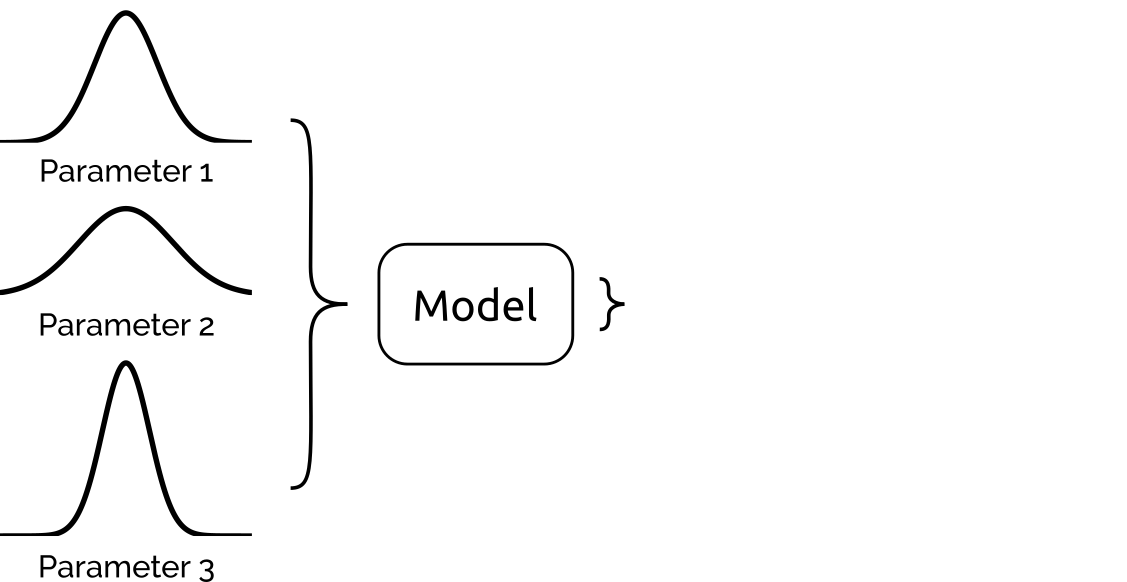
\includegraphics[width=1\textwidth]{mc_1.png}}
    \only<2>{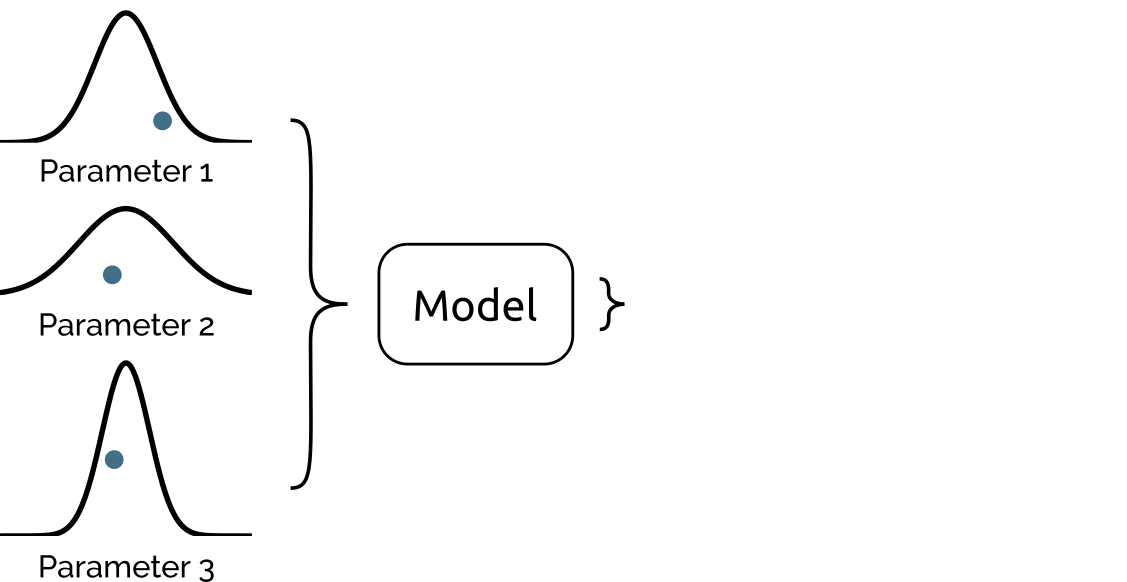
\includegraphics[width=1\textwidth]{mc_2.png}}
    \only<3>{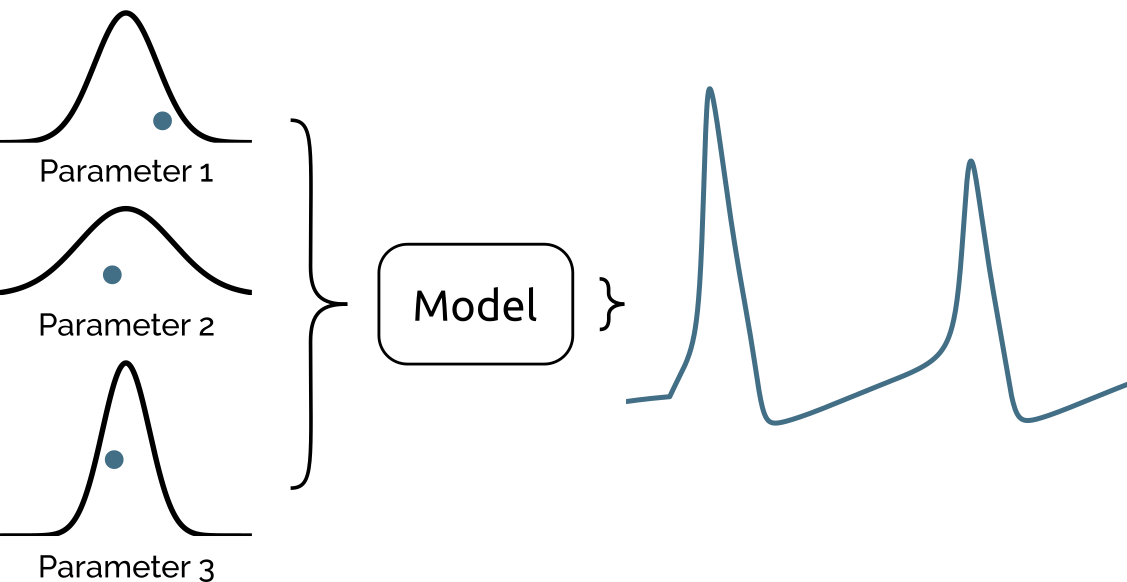
\includegraphics[width=1\textwidth]{mc_3.png}}
    \only<4>{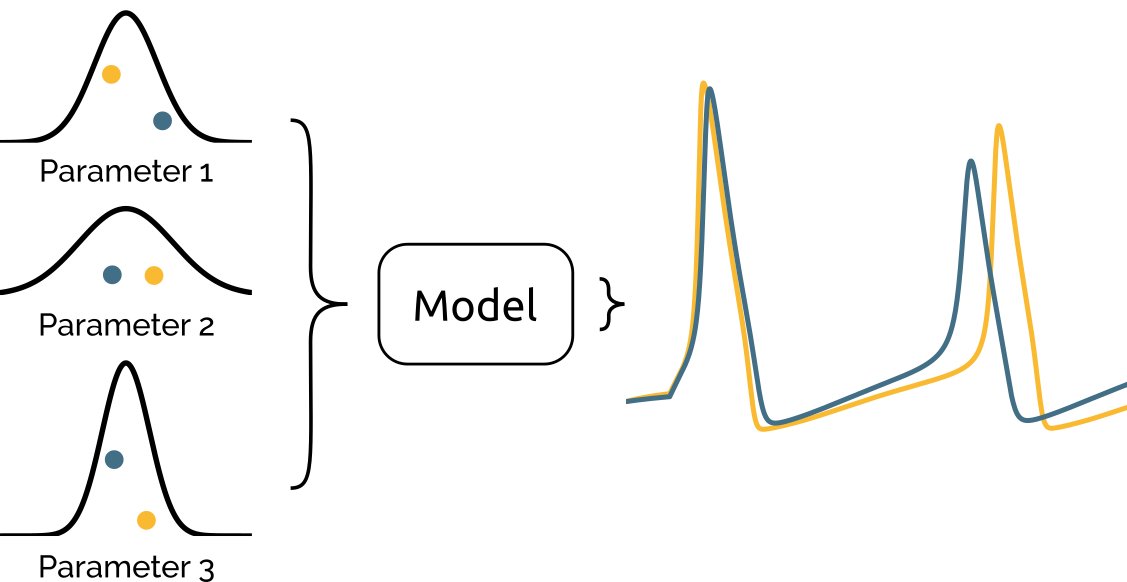
\includegraphics[width=1\textwidth]{mc_4.png}}
    \only<5>{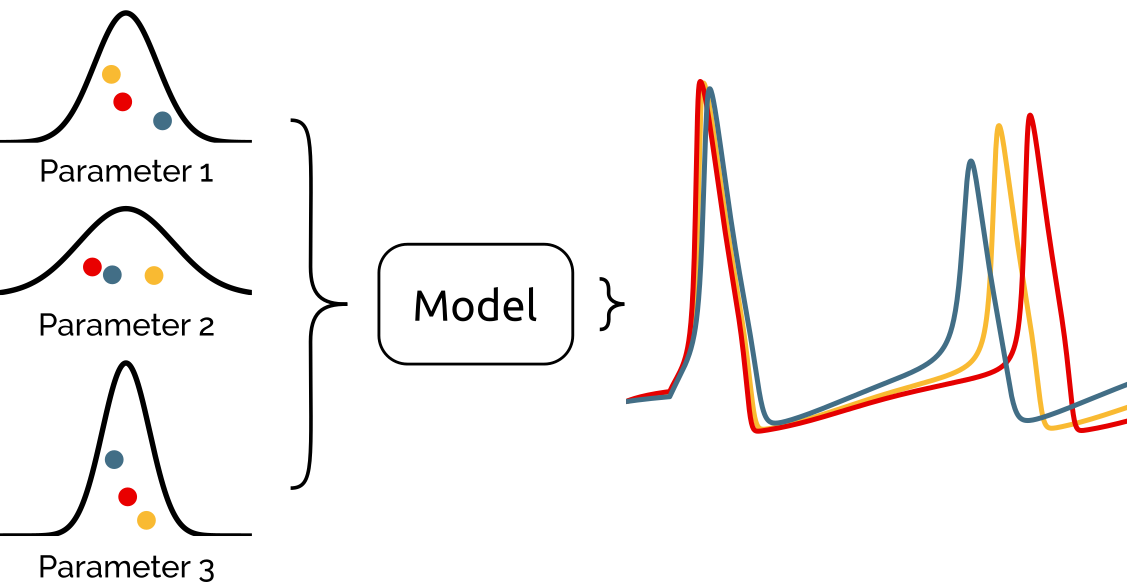
\includegraphics[width=1\textwidth]{mc_5.png}}
  \end{figure}
\end{frame}



\begin{frame}[fragile]
\vspace{-1cm}
\begin{figure}

\includegraphics[width=1\textwidth]{uncertainpy.png}
\end{figure}

{\LARGE \bf A Python toolbox for uncertainty quantification}

\vspace{1cm}

Found at:

\begin{lstlisting}
https://github.com/simetenn/uncertainpy
\end{lstlisting}


Installation:

\begin{lstlisting}
pip install uncertainpy
\end{lstlisting}

\end{frame}


%%%%%%%%%%%%%
%   Frame   %
%%%%%%%%%%%%%

\begin{frame}{Uncertainpy performs all uncertainty calculations and requires the model and parameters}
  \begin{figure}
    \only<1>{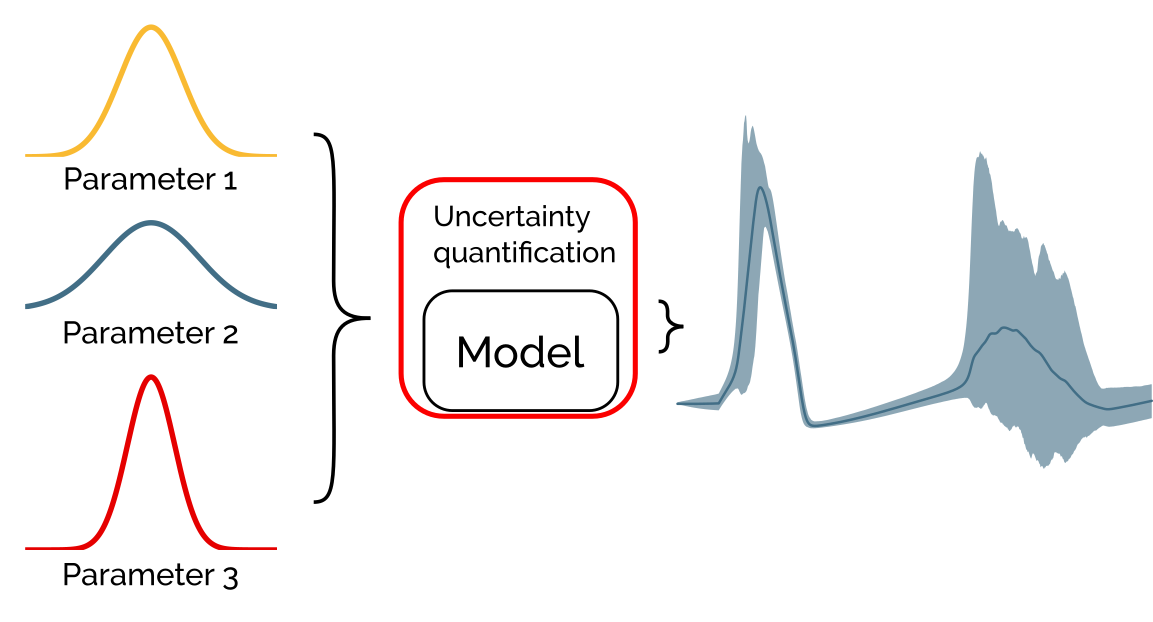
\includegraphics[width=1\textwidth]{probabalistic_un.png}}
    \only<2>{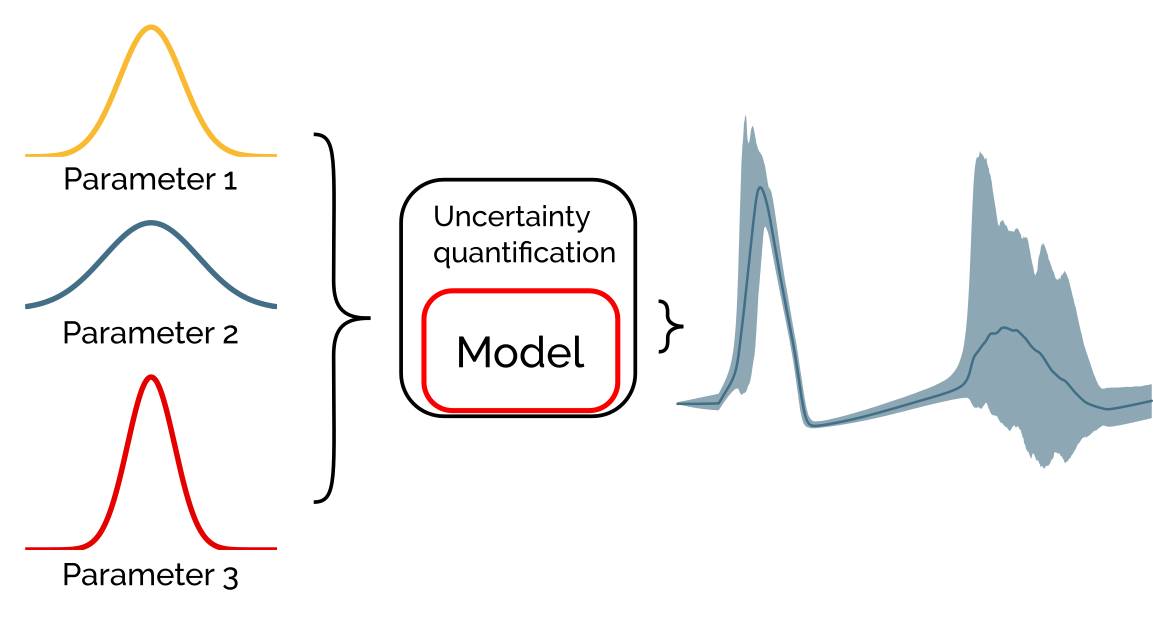
\includegraphics[width=1\textwidth]{probabalistic_model.png}}
    \only<3>{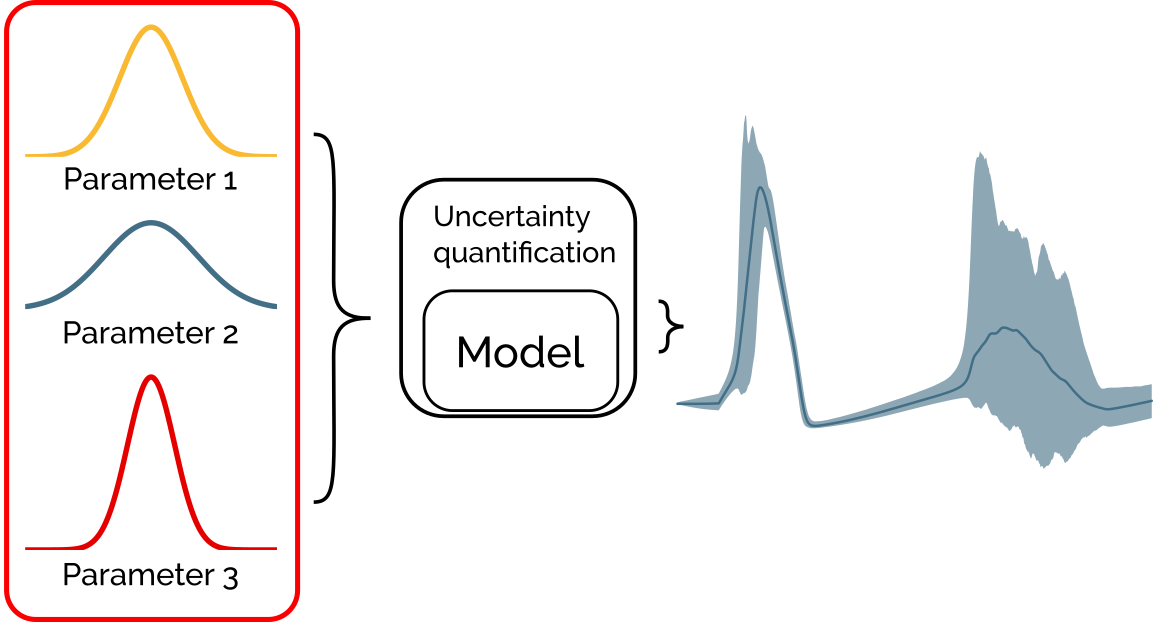
\includegraphics[width=1\textwidth]{probabalistic_parameters.png}}
  \end{figure}
\end{frame}



%%%%%%%%%%%%%
%   Frame   %
%%%%%%%%%%%%%

\begin{frame}[fragile]{The problem is set up using the
            \lstinline|UncertaintyQuantification| class}


  \begin{lstlisting}
import uncertainpy as un

UQ = un.UncertaintyQuantification(
    model=...,
    parameters=...
)
  \end{lstlisting}
  % (*@\texttt{\textcolor{listingsbasiccolor}{\textcolor<3>{red}{parameters}}}@*)
\end{frame}





%%%%%%%%%%%%%
%   Frame   %
%%%%%%%%%%%%%

\begin{frame}[fragile]{Models are created as Python functions}


  \begin{lstlisting}
def hodgin_huxley(gbar_Na, gbar_K, gbar_l):
    # Calculate the membrane potential using
    # gbar_Na, gbar_K and gbar_l

    ...

    return time, membrane_potential
  \end{lstlisting}

\end{frame}


%%%%%%%%%%%%%
%   Frame   %
%%%%%%%%%%%%%

\begin{frame}[fragile]{Uncertainpy has support for multi-compartmental models
  \onslide<2>{and network models}}
  \vspace{-2mm}

  \begin{figure}
    
\includegraphics[height=0.3\textheight]{neuron.jpeg}
  \end{figure}
  \pause
  \begin{figure}
    
\includegraphics[height=0.25\textheight]{nest.png}
  \end{figure}

\end{frame}

%%%%%%%%%%%%%
%   Frame   %
%%%%%%%%%%%%%

\begin{frame}[fragile]{Parameters are given as a Python dictionary}

  \begin{onlyenv}<1>
    \begin{lstlisting}
parameters = {"name": distribution}
    \end{lstlisting}
  \end{onlyenv}

\begin{onlyenv}<2>
    \begin{lstlisting}
import chaospy as cp

uniform_distribution = cp.Uniform(2, 5)
normal_distribution = cp.Normal(12, 2)
    \end{lstlisting}
  \end{onlyenv}

  \begin{onlyenv}<3>
    \begin{lstlisting}
parameters = {                       # Original
  "gbar_Na": cp.Uniform(100, 140),   # 120
  "gbar_K": cp.Uniform(32, 40),      # 36
  "gbar_l": cp.Uniform(0.2, 0.4)     # 0.3
}
    \end{lstlisting}
  \end{onlyenv}
\end{frame}


%%%%%%%%%%%%%
%   Frame   %
%%%%%%%%%%%%%

\begin{frame}[fragile]{We perform the uncertainty calculations with \lstinline|quantify()|}

\begin{lstlisting}
UQ = un.UncertaintyQuantification(
    model=hodgkin_huxley,
    parameters=parameters
)
\end{lstlisting}

\pause

\begin{lstlisting}
results = UQ.quantify()
\end{lstlisting}

\end{frame}





%%%%%%%%%%%%%
%   Frame   %
%%%%%%%%%%%%%



\begin{frame}[fragile]{Overview of the Hodgkin-Huxley example}
\vspace{-3mm}

\begin{lstlisting}
def hodgin_huxley(gbar_Na, gbar_K, gbar_l):
  # Calculate the membrane potential using
  # gbar_Na, gbar_K and gbar_l

  return time, membrane_potential

parameters = {                       # Original
  "gbar_Na": cp.Uniform(100, 140),   # 120
  "gbar_K": cp.Uniform(32, 40),      # 36
  "gbar_l": cp.Uniform(0.2, 0.4)}    # 0.3

UQ = un.UncertaintyQuantification(
    model=hodgkin_huxley,
    parameters=parameters)

results = UQ.quantify()
\end{lstlisting}

\end{frame}


%%%%%%%%%%%%%
%   Frame   %
%%%%%%%%%%%%%

\begin{frame}{90\% prediction interval of the \\ Hodgkin-Huxley model}
  \vspace{-5mm}
  \begin{figure}
    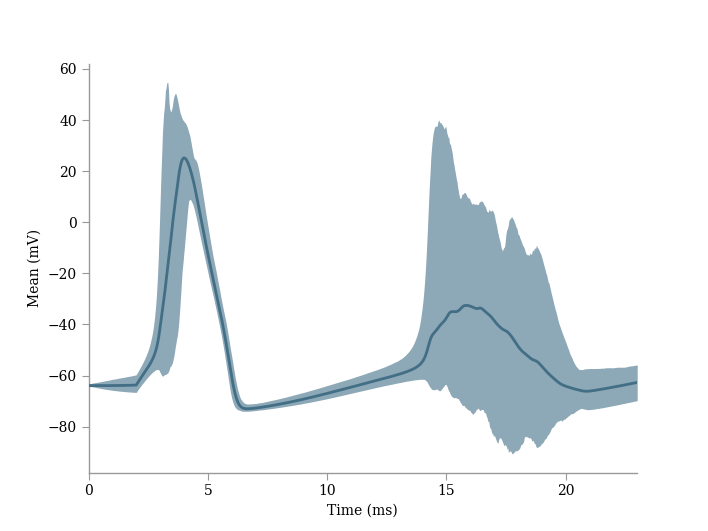
\includegraphics[width=1\textwidth]{hh_prediction.png}
  \end{figure}

\end{frame}



%%%%%%%%%%%%%
%   Frame   %
%%%%%%%%%%%%%

\begin{frame}{Mean and variance of the Hodgkin-Huxley model}
  \vspace{-5mm}
  \begin{figure}
    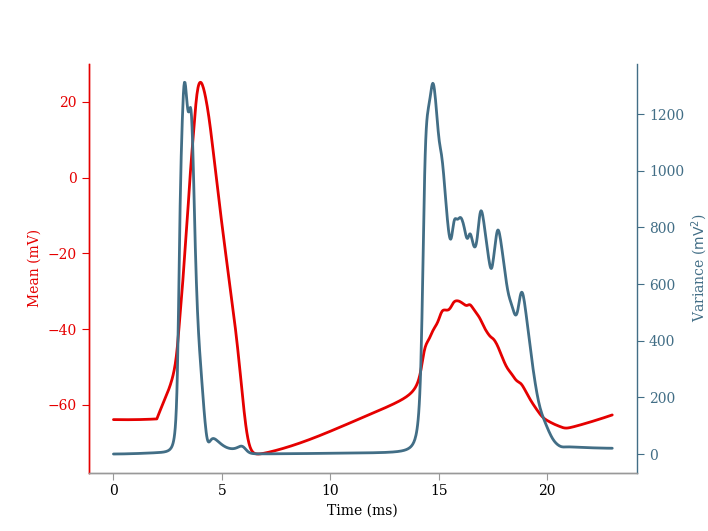
\includegraphics[width=1\textwidth]{hh_mean.png}
  \end{figure}

\end{frame}


%%%%%%%%%%%%%%%%%%%%%%%%%%%%%%%
%                             %
%   What is SA                %
%                             %
%%%%%%%%%%%%%%%%%%%%%%%%%%%%%%%


%%%%%%%%%%%%%
%   Frame   %
%%%%%%%%%%%%%



\begin{frame}{Sensitivity analysis quantifies how much of the uncertainty each
  parameter is responsible for}
\vspace{-5mm}
\begin{figure}
 \only<1>{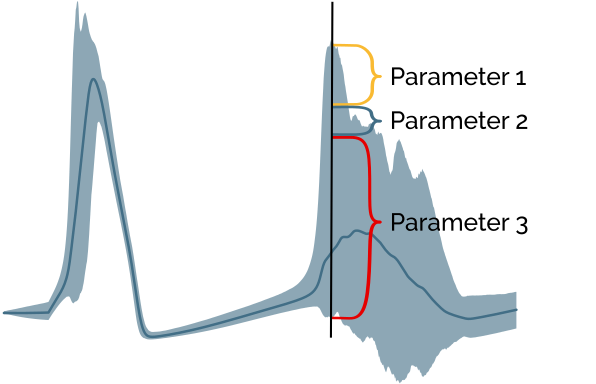
\includegraphics[width=1\textwidth]{sensitivity_explanation_1.png}}
 \only<2>{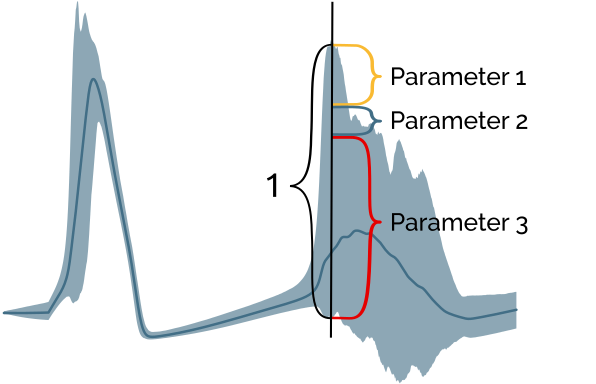
\includegraphics[width=1\textwidth]{sensitivity_explanation_2.png}}
\end{figure}

\end{frame}


%%%%%%%%%%%%%
%   Frame   %
%%%%%%%%%%%%%


\begin{frame}{Sensitivity of the potassium conductance $\overline{g}_{K}$ in the
              Hodgkin-Huxley model}
\vspace{-5mm}
\begin{figure}
  \only<1>{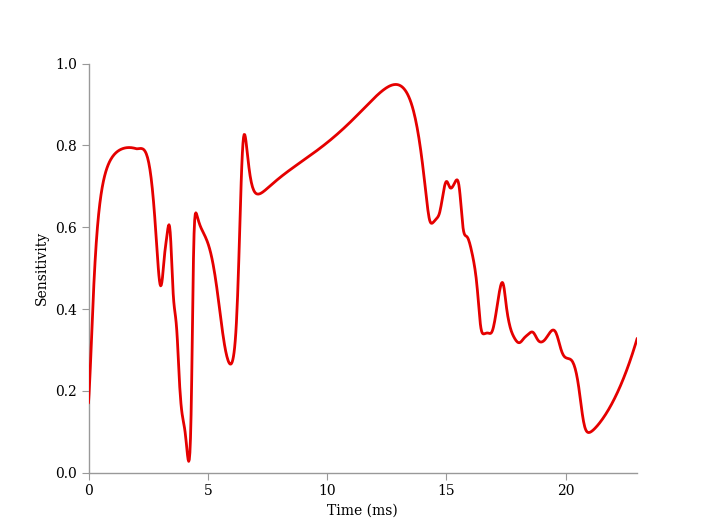
\includegraphics[width=1\textwidth]{sensitivity.png}}
  \only<2>{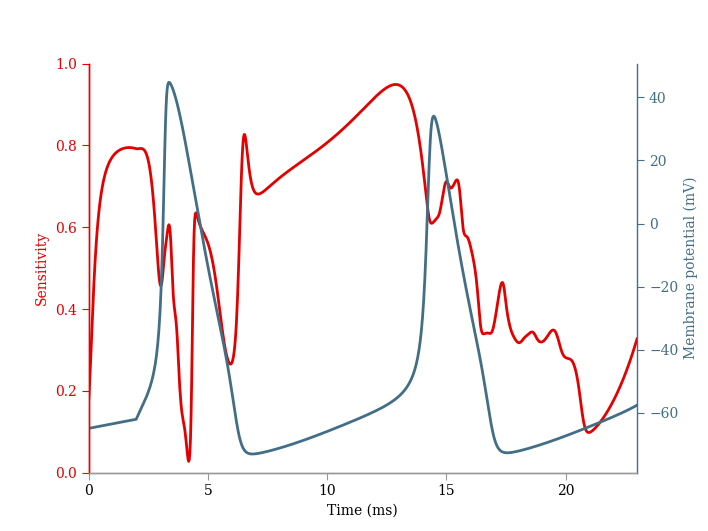
\includegraphics[width=1\textwidth]{sensitivity_mean.png}}
\end{figure}

\end{frame}



%%%%%%%%%%%%%
%   Frame   %
%%%%%%%%%%%%%



\begin{frame}
\begin{figure}
 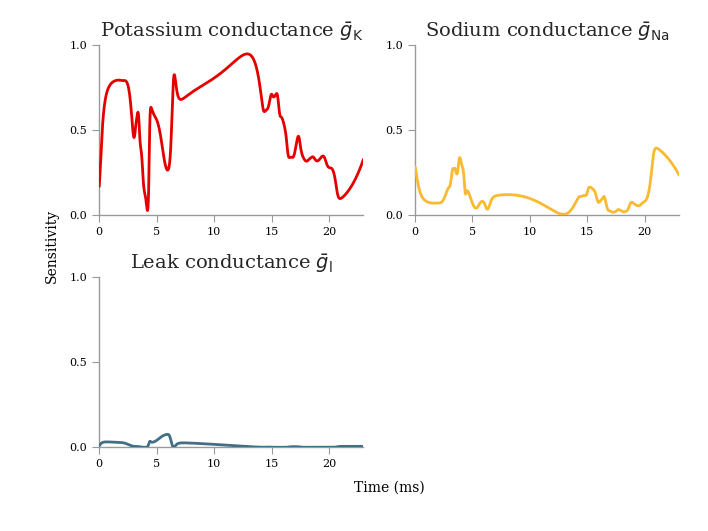
\includegraphics[width=1\textwidth]{sensitivity_all.png}
\end{figure}

\end{frame}


%%%%%%%%%%%%%%%%%%%%%%%%%%%%%%%
%                             %
%   Features                  %
%                             %
%%%%%%%%%%%%%%%%%%%%%%%%%%%%%%%

%%%%%%%%%%%%%
%   Frame   %
%%%%%%%%%%%%%

\begin{frame}

\fullimage{compare.png}{1.4}

\end{frame}


%%%%%%%%%%%%%
%   Frame   %
%%%%%%%%%%%%%



\begin{frame}{Pointwise comparison of model results give large differences
  due to small time shifts in spikes}

  \begin{figure}
   \only<1>{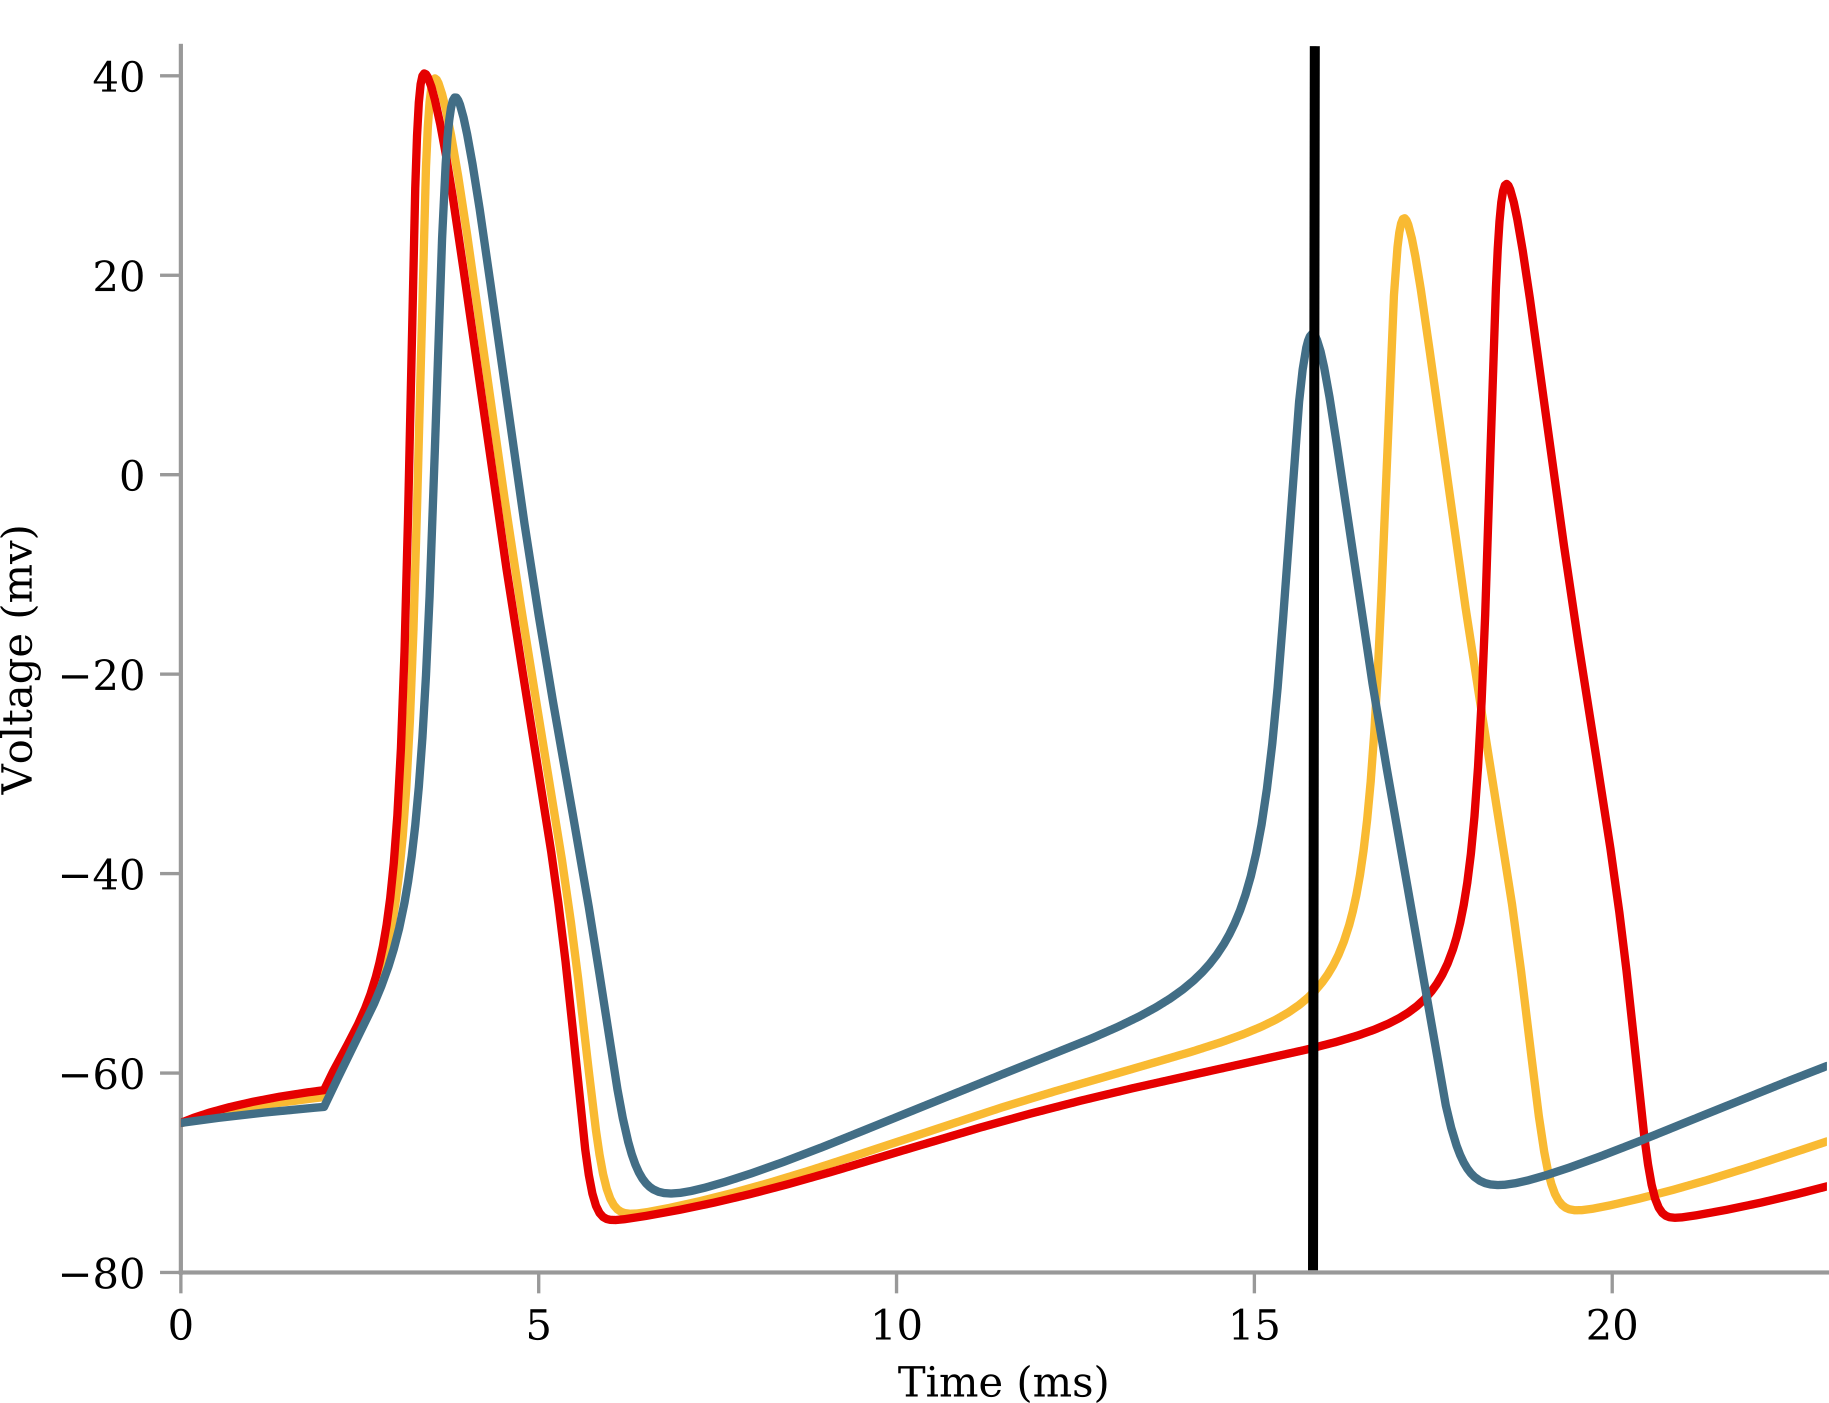
\includegraphics[width=0.8\textwidth]{features_why.png}}
   \only<2>{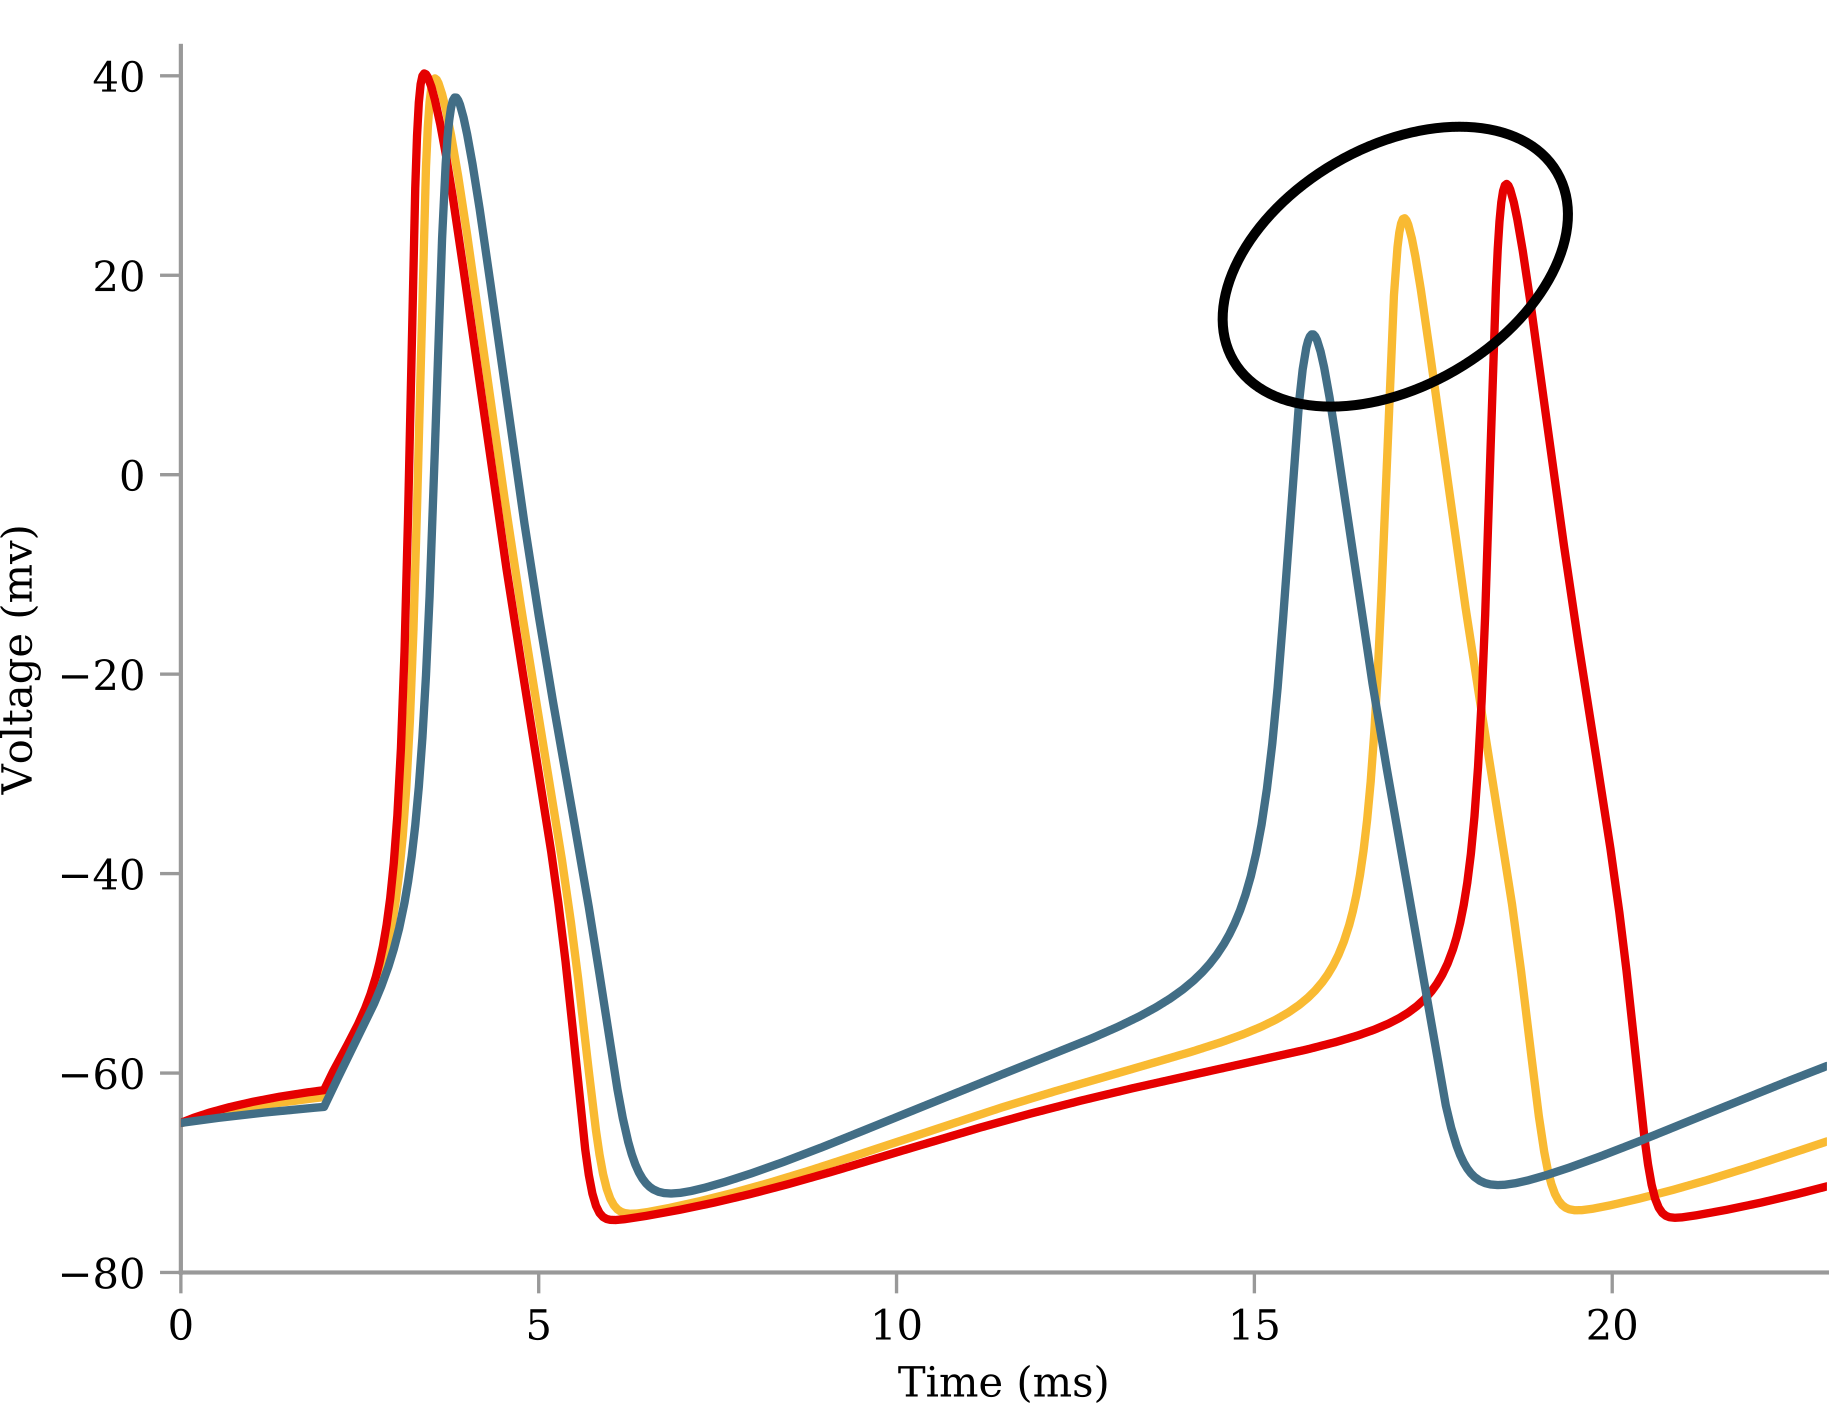
\includegraphics[width=0.8\textwidth]{features_why_2.png}}
   \only<3>{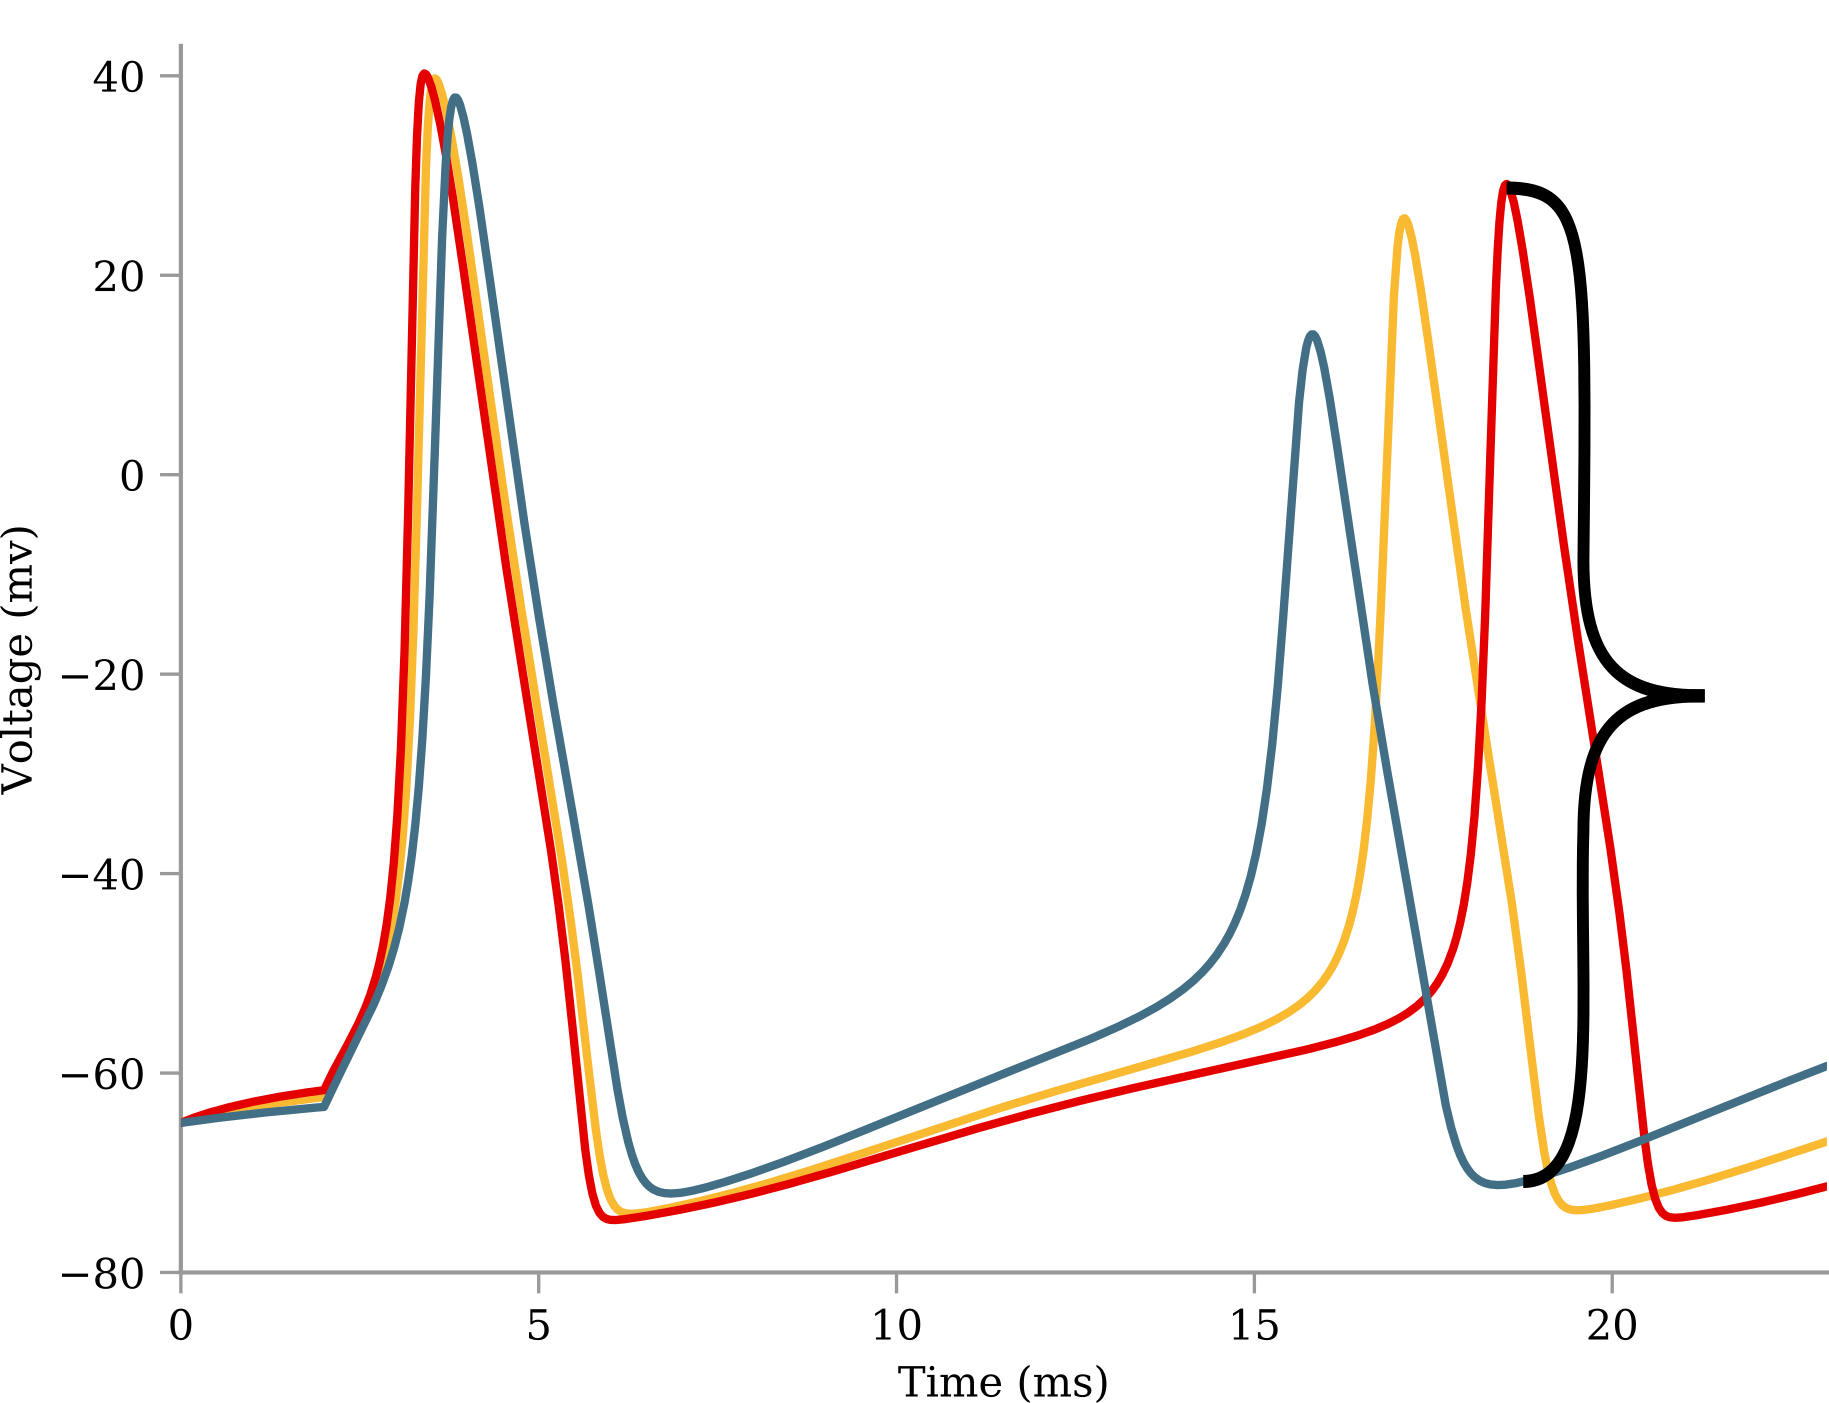
\includegraphics[width=0.8\textwidth]{features_why_3.png}}
  \end{figure}

\end{frame}



%%%%%%%%%%%%%
%   Frame   %
%%%%%%%%%%%%%


\begin{frame}{The time shifted spikes cause large variance}
  \vspace{-5mm}
  \begin{figure}
    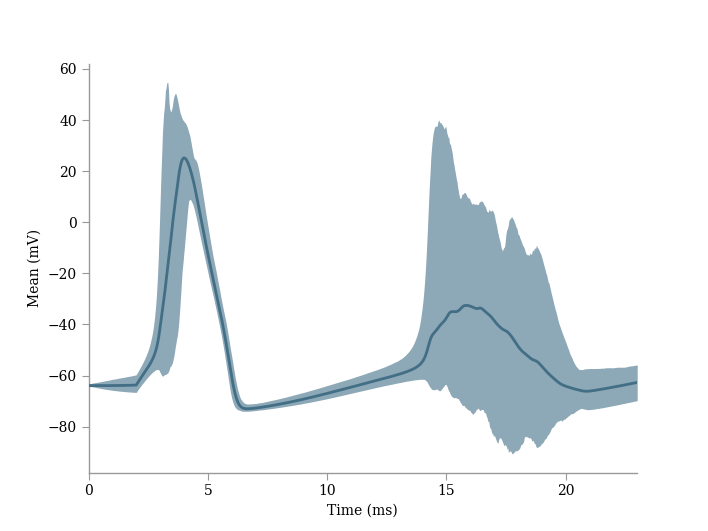
\includegraphics[width=1\textwidth]{hh_prediction.png}
  \end{figure}
  \end{frame}


%%%%%%%%%%%%%
%   Frame   %
%%%%%%%%%%%%%


\begin{frame}{The solution is to compare features of the model,
  such as the number of spikes}
  \vspace{-5mm}
  \begin{figure}
    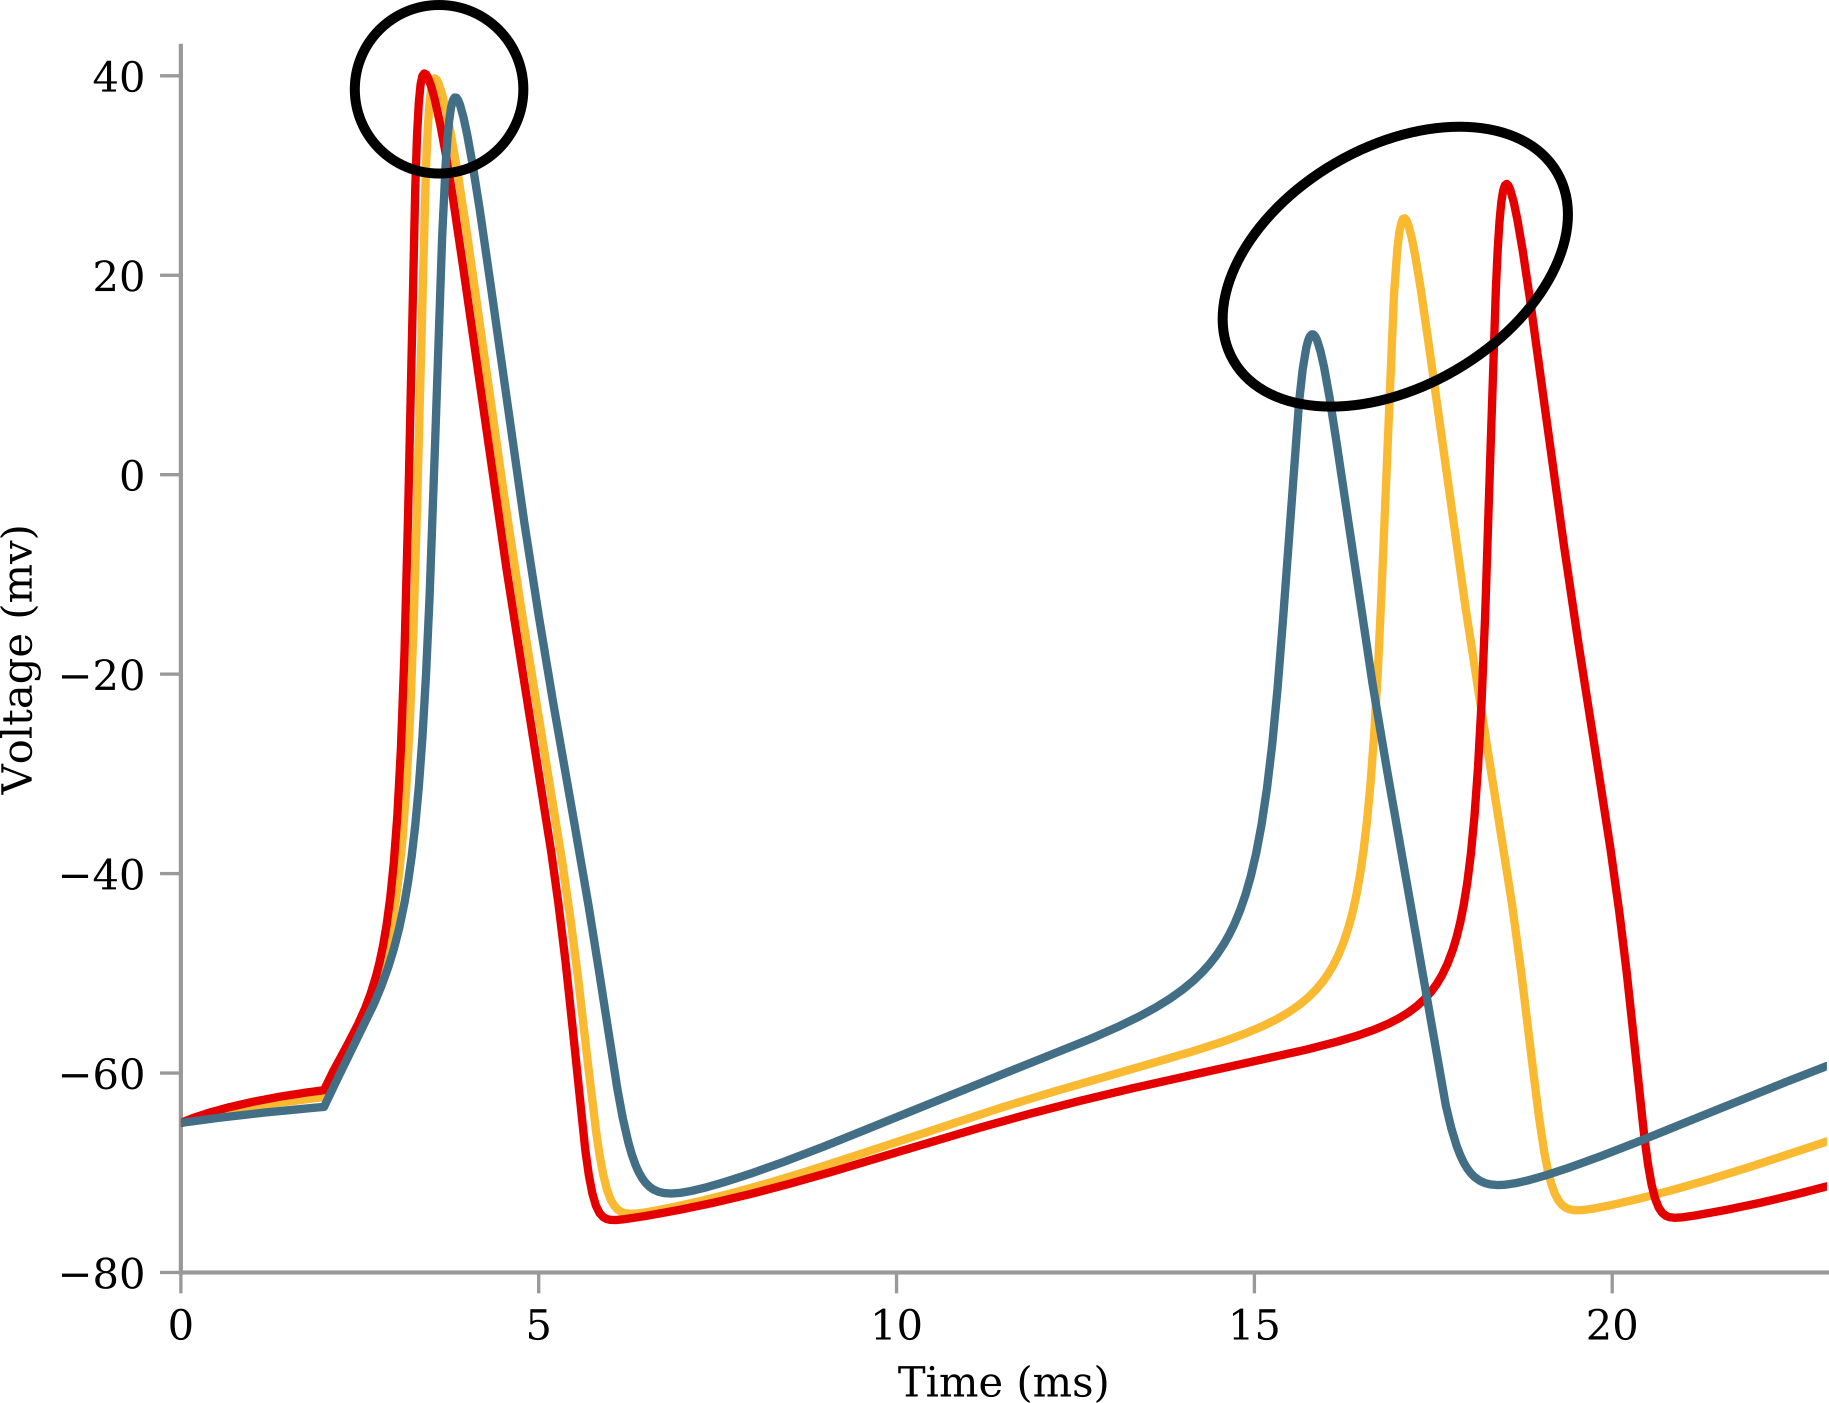
\includegraphics[width=0.8\textwidth]{features_nrspikes.png}
  \end{figure}
  \end{frame}


%%%%%%%%%%%%%
%   Frame   %
%%%%%%%%%%%%%

\begin{frame}{Uncertainpy calculates the uncertainty for a user selected set of
              features of the model}
  \vspace{-5mm}
  \begin{figure}
      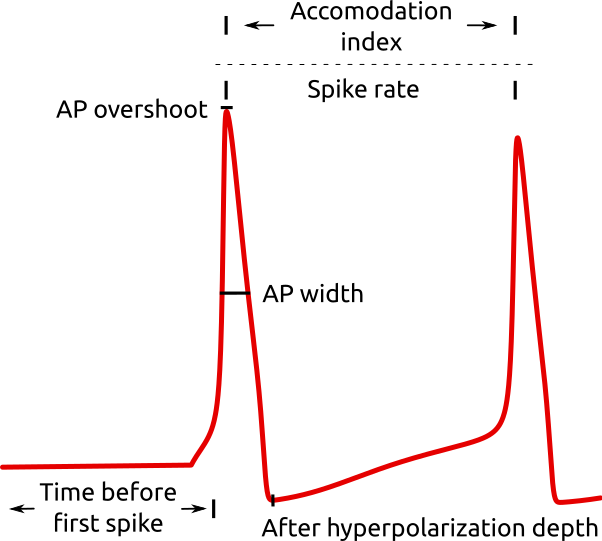
\includegraphics[width=0.7\textwidth]{features.png}
  \end{figure}
  \end{frame}



%%%%%%%%%%%%%
%   Frame   %
%%%%%%%%%%%%%


\begin{frame}[fragile]{Uncertainpy comes with pre-defined features that can be
  directly used with the \lstinline|features| argument}

  \begin{lstlisting}
UQ = un.UncertaintyQuantification(
    model=hodgkin_huxley,
    parameters=parameters,
    features=un.SpikingFeatures()
)
  \end{lstlisting}


\end{frame}



%%%%%%%%%%%%%
%   Frame   %
%%%%%%%%%%%%%

\begin{frame}[fragile]{Features are defined as Python functions}

  \begin{lstlisting}
def nr_spikes(time, membrane_potential):
    # Calculate the feature using
    # time and membrane_potential

    ...

    return time, nr_spikes
  \end{lstlisting}

\end{frame}

%%%%%%%%%%%%%
%   Frame   %
%%%%%%%%%%%%%

\begin{frame}[fragile]{A list of feature functions is given with the
  \lstinline|features| argument}

  \begin{lstlisting}
UQ = un.UncertaintyQuantification(
    model=hodgkin_huxley,
    parameters=parameters,
    features=[nr_spikes, feature_function_2]
)
  \end{lstlisting}
\end{frame}






%%%%%%%%%%%%%
%   Frame   %
%%%%%%%%%%%%%


\begin{frame}{{\normalsize Summary:} \\ Uncertainty quantification enables us to take the
  effects of uncertain parameters into account}

\pause
  % First point
  \begin{tikzpicture}[remember picture, overlay, font=\sffamily]
    \node [align=left, xshift=-3.3cm, yshift=1cm] (image3) at (current page.center)
          {\includegraphics[width = 0.45\textwidth]{uncertainpy.png}};
  \end{tikzpicture}

  \begin{tikzpicture}[remember picture, overlay, font=\sffamily]
    \node[align=left, xshift=-0.3cm, yshift=1cm, anchor=west] at (current page.center) {\bf performs all calculations without \\ \bf the need for detailed knowledge};
  \end{tikzpicture}

  \pause
  % Second point
  \begin{tikzpicture}[remember picture, overlay, font=\sffamily]
    \node [align=left, xshift=-3.3cm, yshift=-1.9cm] (image1) at (current page.center)
        {\includegraphics[width = 0.32\textwidth]{features_nrspikes.png}};
    \end{tikzpicture}

    \begin{tikzpicture}[remember picture, overlay, font=\sffamily]
      \node[align=left, xshift=-0.3cm, yshift=-1.9cm, anchor=west] at (current page.center) {\bf Features are useful when\\ \bf comparing spiking results};
    \end{tikzpicture}




     \begin{tikzpicture}[remember picture, overlay, font=\sffamily]
         \node [align=left, xshift=0.49\textwidth,yshift=-0.37\textwidth] (image2) at (current page.center)
               {\includegraphics[width = 0.3\textwidth]{cinpla.png}};
       \end{tikzpicture}


  \pause
  \begin{tikzpicture}[remember picture, overlay, font=\sffamily]

    \node[align=left, yshift=0.07\textwidth] at (current page.south){ \bf \large Questions?};
  \end{tikzpicture}

\end{frame}



\end{document}
